%!TEX TS-program = xelatex

%!TEX root = ../Thesis.tex

% This information is used in titlepage, colophon, preface and hyperref setup (pdf metainfo), and other options.

%\def\thesistypeabbr{B.Eng.}
%\def\thesistype    {Bachelor of Engineering}
%\def\thesistypeabbr{B.Sc.Eng.}
%\def\thesistype    {Bachelor of Science in Engineering}
%\def\thesistypeabbr{M.Sc.}
%\def\thesistype    {Master of Science in Engineering}
\def\thesistypeabbr{Ph.D.}
\def\thesistype    {Doctor of Philosophy}

\def\thesisauthor  {Søren Vind}
%\def\thesistitle   {Assorted Adventures in Data Structures}
%\def\thesissubtitle{For Strings and Range Searching}
%\def\thesistitle   {Advances in Data Structures}
%\def\thesissubtitle{Points on Strings and Strings about Points}

%\def\thesistitle   {Adventures in Data Structures}
%\def\thesissubtitle{Points about Strings and Strings about Points}
%\def\thesistitle   {Points about Strings and Strings about Points}
%\def\thesissubtitle{Algorithms and Data Structures for Strings and Range Searching}
%\def\thesistitle{Points about Strings and Strings about Points}
%\def\thesissubtitle{Algorithms and Data Structures for Text and Range Searching}

\def\thesistitle{Algorithms and Data Structures \\for Strings, Points and Integers}
\def\thesissubtitle{Points about Strings and Strings about Points}

\def\thesislocation{Copenhagen}
\def\thesisnumber{PHD-2015-366}
\def\thesisISSN{0909-3192}

\def\papersize    {b5paper} % Final papersize (b5paper/a4paper), recommended papersize for DTU Compute is b5paper
\def\showtrims    {false} % Print on larger paper than \papersize and show trim marks (true/false)?

\def\showtodos    {true}  % Show todos (true/false)?
\def\confidential {false} % Confidential thesis (true/false)?


\input{preamble/general}
\input{preamble/fonts}
\input{preamble/etc}
%!TEX root = ../Thesis.tex

%% TIKZ
\usetikzlibrary{decorations.pathreplacing}
\usetikzlibrary{decorations.pathmorphing}
\usetikzlibrary{calc}
\usetikzlibrary{shapes.geometric}
\usetikzlibrary{shapes.misc}
\usetikzlibrary{positioning}
\usetikzlibrary{patterns}
\usetikzlibrary{fit}
\usetikzlibrary{arrows}
\usetikzlibrary{decorations.markings}
\usetikzlibrary{matrix}
\tikzstyle{every picture}+=[remember picture]


\usepackage[english]{babel}
\usepackage{upgreek}
\usepackage{amsthm,amsmath,nicefrac,graphicx,lastpage,array}
%,amssymb
 

\newtheorem{theorem}{Theorem}[section]
\newtheorem{corollary}{Corollary}[theorem]
\newtheorem{lemma}[theorem]{Lemma}
\newtheorem{definition}{Definition}
\newtheorem{fact}{Fact}


\frenchspacing


 
%%%%%%%%%%%%%%%%%%%%%%%%%%%%%%%%%%%%%%%%%%%
% Proper and meaningful colored Fixmes.
% Simpler interface to fixmes/todos
\usepackage{soul} % provides sethlcolor, hl for fixes
\usepackage{framed} % shading for notes
\definecolor{shadecolor}{rgb}{1,0.8,0.2} % shade color for notes
%\definecolor{shadecolor}{rgb}{1,0.8,0.2} % shade color for notes

\usepackage[inline,nomargin,author=,draft]{fixme}
\fxusetheme{color}
%\fxsetface{inline}{\bfseries}
%\fxsetface{inline}{\rmfamily}
%\newcommand{\note}[1]{\fxnote{\hlc[gray!0.2]{#1}}}
\newcommand{\note}[1]{\begin{shaded}\fxnote{#1}\end{shaded}}
\renewcommand{\todo}[1]{\begin{shaded}\fxfatal{#1}\end{shaded}}

\newcommand{\hlc}[2][yellow]{{\sethlcolor{#1} \hl{#2}}}
\newcommand{\fix}[1]{\fxfatal{\hlc[yellow]{#1}}}
\newcommand{\docite}[1]{\footnote{\fix{#1}}}
%%%%%%%%%%%%%%%%%%%%%%%%%%%%%%%%%%%%%%%%%%%




%%%%%%%%%%%%%%%%%%%%%%%%%%%%%%%%%%%%%%%%%%%
%%%%%%%%%%%%%%%%%% Info about papers
\newenvironment{infosection}
    {}
    {\clearpage}
\newcommand{\published}[1]{\noindent {\paragraph{Publication} #1}}
%\newenvironment{authors}
%    {\begin{center}}
%    {\end{center}\setcounter{footnote}{0}\vspace{1em}}
    \newenvironment{authors}
      {\vspace{1cm}\par\edef\savedfootnotenumber{\number\value{footnote}}
       \renewcommand{\thefootnote}{\fnsymbol{footnote}}
       \setcounter{footnote}{0}\centering}
      {\par\setcounter{footnote}{\savedfootnotenumber}}
    
\newenvironment{uninames}
    {\begin{center}}
    {\end{center}\vspace{3em}}



\makeatletter
\def\@xfootnote[#1]{%
  \protected@xdef\@thefnmark{#1}%
  \@footnotemark\@footnotetext}
\makeatother

%% Specify affiliations with this massive hack
%\newcommand{\uniname}[2]{\footnotemark[#1] #2 \\}
\newcommand{\uni}[1]{$^{#1}$}
\newcommand*\samethanks[1][\value{footnote}]{\footnotemark[#1]}
%%%%%%%%%%%%%%%%%%%%%%%%%%%%%%%%%%%%%%%%%%%


% Table row height. From IEEE package documentation
\renewcommand{\arraystretch}{1.2}


%%%%%%%%%%%%%%% MAKES AUTHORS ON TOP WITH MAKETITLE.
\begin{comment}
%%% FROM LIPICS
\makeatletter
\renewcommand\maketitle{\par
  \begingroup
    \renewcommand\thefootnote{\@fnsymbol\c@footnote}%
    \if@twocolumn
      \ifnum \col@number=\@ne
        \@maketitle
      \else
        \twocolumn[\@maketitle]%
      \fi
    \else
      %\newpage
      \global\@topnum\z@   % Prevents figures from going at top of page.
      \@maketitle
    \fi
    \thispagestyle{plain}\@thanks
  \endgroup
  \setcounter{footnote}{0}%
  \global\let\thanks\relax
  \global\let\maketitle\relax
  \global\let\@maketitle\relax
  \global\let\@thanks\@empty
  \global\let\@author\@empty
  \global\let\@date\@empty
  \global\let\@title\@empty
  \global\let\title\relax
  \global\let\author\relax
  \global\let\date\relax
  \global\let\and\relax
}
\def\@maketitle{%
  %\newpage
  %\null\vskip-\baselineskip
  %\vskip-\headsep
  \let \footnote \thanks
  \parindent\z@ \raggedright
    \ifnum\c@authors=0 %
      \@latexerr{No \noexpand\author given}%
        {Provide at least one author. See the LIPIcs class documentation.}%
    \else
      \@author
    \fi
  \par}
\makeatother

\usepackage{authblk}
\renewcommand*\Authand{{ and }}
\end{comment}


%!TEX root = ../Thesis.tex


\newcommand{\prob}[1]{\emph{#1}}
\newcommand{\paper}[1]{\emph{#1}}

%%%%%%%%%%%%%%%%%%%%%%%%%%%%%%%%%%%%%%%%%%%%%%%%%%%%%%%%%%
%%%%%%%%%%%%%%%%%% Fingerprints
%%%%%%%%%%%%%%%%%%%%%%%%%%%%%%%%%%%%%%%%%%%%%%%%%%%%%%%%%%

%Macros: Queries
\newcommand{\fingerprintq}{\ensuremath{\textsc{Fingerprint}}}
\newcommand{\lceq}{\ensuremath{\textsc{LCE}}}
\newcommand{\levelanc}{\ensuremath{\textsc{LA}}}
\renewcommand{\succ}{\ensuremath{\textsc{succ}}}
\newcommand{\pred}{\ensuremath{\textsc{pred}}}

%Macros: Fingerprints
\newcommand{\fp}{\ensuremath\phi}
\newcommand{\fpv}{\ensuremath{\phi_v}}
\newcommand{\fpe}{\ensuremath{\phi_e}}
\newcommand{\fpplus}{\ensuremath{\oplus}}
\newcommand{\fpdelsuffix}{\ensuremath{\ominus_s}}
\newcommand{\fpdelprefix}{\ensuremath{\ominus_p}}

%Macros: Trees, SLPs
\newcommand{\size}{\ensuremath{\mathit{size}}}
\newcommand{\depth}{\ensuremath{\mathit{depth}}}
\newcommand{\leaf}{\ensuremath{\mathit{leaf}}}
\newcommand{\heavy}{\ensuremath{heavy}}
\newcommand{\heavypath}{\ensuremath{H}}
\newcommand{\rootnode}{\ensuremath{\mathit{root}}}
\newcommand{\lchild}{\ensuremath{\mathit{left}}}
\newcommand{\rchild}{\ensuremath{\mathit{right}}}
\newcommand{\leftnodes}{\ensuremath{V}} %V
\newcommand{\leftsize}{\ensuremath{L}} %L
\newcommand{\leftstring}{\ensuremath{P}} %P
\newcommand{\str}{\ensuremath{S} }
\newcommand{\slp}{\ensuremath{G} }
\newcommand{\lslp}{\ensuremath{G_L} }

%Macros: Misc
\newcommand{\lce}{\ensuremath\ell}
\newcommand{\rs}{root-substring}



%%%%%%%%%%%%%%%%%%%%%%%%%%%%%%%%%%%%%%%%%%%%%%%%%%%%%%%%%%
%%%%%%%%%%%%%%%%%% Pattern Extraction
%%%%%%%%%%%%%%%%%%%%%%%%%%%%%%%%%%%%%%%%%%%%%%%%%%%%%%%%%%

\renewcommand{\epsilon}{\upvarepsilon}

%Functions/Operators
\newcommand{\suff}{\operatorname{suffix}}
\newcommand{\prefset}{\operatorname{prefset}}
\newcommand{\maxpref}{\operatorname{maxprefix}}
\newcommand{\lab}{\operatorname{label}}
\newcommand{\srt}{\operatorname{sort}}
\newcommand{\argmax}{\operatornamewithlimits{argmax}}

% NEW COMMANDS FOR MOTIFS
\newcommand{\calph}{\Sigma} % Alphabet for characters
\newcommand{\salph}{\Pi} % Alphabet for solid blocks

\newcommand{\lexleq}{\preceq_{lex}}
\newcommand{\lexl}{\prec_{lex}}

\newcommand{\dontcare}{\star}
\newcommand{\numdc}{\operatorname{dc}}
\newcommand{\occ}{\operatorname{occ}}
\newcommand{\ilcp}{\operatorname{LCP}}
\newcommand{\lcp}{\operatorname{\textit{lcp}}}
\newcommand{\reverse}{\operatorname{reverse}}
\newcommand{\maxlcp}[1]{\operatorname{\ell}_{#1}}
\newcommand{\occs}[1]{L_{#1}}
\newcommand{\sortoccs}[1]{E_{#1}}
\newcommand{\interval}[1]{I_{#1}}
\newcommand{\intervalset}[1]{\mathcal{I}_{#1}}
\newcommand{\handlevalset}[1]{\mathcal{H}_{#1}}
\newcommand{\maxset}{\mathcal{M}}
\newcommand{\nummax}{|\mathcal{M}|}

\newcommand{\rintset}{\mathcal{R}}
\newcommand{\candset}{\mathcal{C}}

\newcommand{\generate}[1]{\operatorname{\textsc{Generate}}\ensuremath{(#1)}}

% EXTENSIONS
\newcommand{\ext}{\operatorname{ext}}
\newcommand{\skipchar}{\operatorname{skip}}
\newcommand{\skipset}[1]{P_{#1}}

\newcommand{\istart}[1]{\operatorname{start}(#1)}
\newcommand{\iend}[1]{\operatorname{end}(#1)}





%%%%%%%%%%%%%%%%%%%%%%%%%%%%%%%%%%%%%%%%%%%%%%%%%%%%%%%%%%
%%%%%%%%%%%%%%%%%% Colored Range Counting
%%%%%%%%%%%%%%%%%%%%%%%%%%%%%%%%%%%%%%%%%%%%%%%%%%%%%%%%%%


%Macros: Trees, SLPs
\newcommand{\bitzero}{\ensuremath{\mathtt{0}}}
\newcommand{\bitone}{\ensuremath{\mathtt{1}}}

%Macros: Points
\newcommand{\points}{\ensuremath{\mathit{points}}}


%Macros: Polylogs
\renewcommand{\log}{\lg}
\newcommand{\polylog}{\ensuremath{\mathrm{\, polylg \,}}}


%Operations
\newcommand{\opins}{\ensuremath{\textsc{insert}}}
\newcommand{\opdel}{\ensuremath{\textsc{delete}}}



%%%%%%%%%%%%%%%%%%%%%%%%%%%%%%%%%%%%%%%%%%%%%%%%%%%%%%%%%%
%%%%%%%%%%%%%%%%%% Compressed Range Searching
%%%%%%%%%%%%%%%%%%%%%%%%%%%%%%%%%%%%%%%%%%%%%%%%%%%%%%%%%%

%Macros: Trees, SLPs
% As above

%Ranges
\newcommand{\range}[1]{\ensuremath{\mathit{r_{#1}}}}
\newcommand{\offset}{\ensuremath{\mathit{offset}}}
\newcommand{\position}{\ensuremath{\mathit{position}}}
\newcommand{\rangespan}{\ensuremath{\mathit{extent}}}

%Macros: Points, Clusters
\newcommand{\rootpath}{\ensuremath{\mathit{path}}}
\newcommand{\rank}{\ensuremath{\mathit{rank}}}
\newcommand{\mindist}{\ensuremath{\mathit{mindist}}}
\newcommand{\maxdist}{\ensuremath{\mathit{maxdist}}}
\newcommand{\vlabel}{\ensuremath{\mathit{label}}}
\newcommand{\diameter}{\ensuremath{\mathit{diameter}}}
\newcommand{\clustering}{\ensuremath{\mathit{C}}}
\newcommand{\inrange}{\ensuremath{\subseteq}}
\newcommand{\height}{\ensuremath{\mathit{height}}}


%%%%%%%%%%%%%%%%%%%%%%%%%%%%%%%%%%%%%%%%%%%%%%%%%%%%%%%%%%
%%%%%%%%%%%%%%%%%% Motion Detection
%%%%%%%%%%%%%%%%%%%%%%%%%%%%%%%%%%%%%%%%%%%%%%%%%%%%%%%%%%

\newcommand{\mdquery}{\ensuremath{\mathtt{MD(T, A, v, p)}}}







%%%%%%%%%%%%%%%%%%%%%%%%%%%%%%%%%%%%%%%%%%%%%%%%%%%%%%%%%%
%%%%%%%%%%%%%%%%%% Annotated
%%%%%%%%%%%%%%%%%%%%%%%%%%%%%%%%%%%%%%%%%%%%%%%%%%%%%%%%%%
\newcommand{\qindex}{\ensuremath{\mathtt{index}}}
\newcommand{\attach}{\ensuremath{\mathtt{attach}}}
\newcommand{\recover}{\ensuremath{\mathtt{recover}}}
\newcommand{\parent}{\ensuremath{parent}}
\newcommand{\sub}{\ensuremath{\mathtt{sub}}}
\newcommand{\tpref}{\ensuremath{\mathtt{tpref}}}
\newcommand{\ppref}{\ensuremath{\mathtt{pref}}}
\newcommand{\len}{\ensuremath{\mathtt{len}}}
\newcommand{\match}{\ensuremath{\mathtt{match}}}
\newcommand{\concat}{\circ}

\newcommand{\lca}{\ensuremath{lca}}

\newcommand{\True}{\ensuremath{\textsc{True}}}
\newcommand{\False}{\ensuremath{\textsc{False}}}


\addbibresource{bibliography/Bibliography.bib}

\begin{document}

\prefrontmatter
%!TEX root = ../Thesis.tex 
\thispagestyle{empty}             % No page numbers
\calccentering{\unitlength}
\begin{adjustwidth*}{\unitlength}{-\unitlength}
    \begin{adjustwidth}{-0.5cm}{-0.5cm}
%        \sffamily%
        \includegraphics[width=0.75\textwidth]{DTU-Compute-B-UK}\\*[0.5cm]
%        \vspace{-2.5em}
%        \begin{flushright}
%            
%            \thesistype{}\\
%        \end{flushright}
%        \vspace*{\fill}
        \vfill
{        
        \centering
        \Huge \thesistitle{}\\*[0.4cm]
        \LARGE \emph{or,}\\*[0.4cm]
        \thesissubtitle{}\\*[1cm]
}
        \vspace{2cm}
        \parbox[b]{0.5\linewidth}{%
            \large 
            \thesisauthor{}\\*[1.2cm]
            {
            \small
            %\thesislocation{} \the\year\\
            \thesistypeabbr{} Thesis\\[0cm]
            \thesisnumber{}\\[0cm]
            ISSN: \thesisISSN{}
            }
        }
        \hfill\includegraphics[scale=0.7]{DTU-logo-CMYK}
    \end{adjustwidth}
\end{adjustwidth*}
\normalfont
\normalsize

\cleartoevenpage
%!TEX root = ../Thesis.tex
\thispagestyle{empty} % No page numbers
\frieze
\vspace*{\fill}
\noindent
\sffamily
\scriptsize
\textbf{DTU Compute}\\
\textbf{Department of Applied Mathematics and Computer Science}\\
\textbf{Technical University of Denmark}\\
\\
Richard Petersens Plads\\
Building 324\\
2800 Kongens Lyngby, Denmark\\
Phone +45 4525 3031\\
compute@compute.dtu.dk\\
www.compute.dtu.dk\\
\\
\thesisnumber{}\\
ISSN: \thesisISSN{}\\
\normalsize
\normalfont
\vspace*{0.5cm}

\clearforchapter

\frontmatter
%!TEX root = ../Thesis.tex
\chapter{Abstract}
\note{Write English Abstract}

%!TEX root = ../Thesis.tex
\chapter{Resumé}
Denne afhandling præsenterer vor forskning i feltet algoritmer og datastrukturer. Mere specifikt viser vi løsninger til følgende problemer relateret til strenge, punkter og heltal. Vores grænser gælder i RAM-modellen, og vi måler plads i antal $w$-bit ord.


\paragraph{Komprimerede Fingeraftryk.}
En strengs Karp-Rabin fingeraftryk er en brugbar type hash-værdi, der har talrige anvendelser på grund af dens stærke egenskaber.
Givet en streng $S$ af længde $N$ komprimeret som et Straight Line Program (SLP) af størrelse $n$, viser vi en datastruktur der kræver $\Oh(n)$ plads som understøtter \emph{fingeraftryksforespørgsler} der returnerer fingeraftrykket af en given delstreng i $S$.
Vi svarer på forespørgsler i $\Oh(\log N)$ tid. Hvis kompressionen er en Lineær SLP (dette omfatter LZ78 kompression og varianter) kan vi svare i $\Oh(\log \log N)$ tid.

Vores løsning matcher den bedst kendte tidsgrænse for at tilgå et enkelt tegn i SLPer, og det er den første for generelle (ikke-balancerede) SLPer der svarer på forespørgsler uden at dekomprimere noget tekst. 
Vi understøtter også \emph{længste fælles delstreng} forespørgsler, der returnerer længden $\ell$ som $S$ matcher sig selv startende fra to givne positioner. 
Vi svarer forespørgsler korrekt med høj sandsynlighed i tid $\Oh(\log N \log \ell)$ og $\Oh(\log \log N + \log \ell \log \log \ell)$ for henholdsvis SLPer og Lineære SLPer.


\paragraph{Dynamisk Kompression.}
I \emph{dynamisk relativ kompression} komprimerer vi en streng $S$ af længde $N$ som $n$ delstrenge fra en given referencestreng af længde $r$.
Vi giver datastrukturer der vedligeholder en asymptotisk optimal kompression i denne model og understøtter operationer der tilgår, ændrer, indsætter og sletter tegn i $S$. 
Vores løsninger understøtter hver operation i $\Oh(\log n / \log \log n + \log \log r)$ tid og $\Oh(n+r)$ plads; eller $\Oh(\log n / \log \log n)$ tid og $\Oh(n+r \log^{\epsilon} r)$ plads.
De generaliserer naturligt til at opbevare flere strenge.

Vi opnår næsten-optimale grænser, og vores løsning er den første der understøtter at dynamisk vedligeholde en streng i en type kompression der kan opnå bedre end entropi-kompression.
Som en del af vores løsning viser vi forbedrede grænser for \emph{delstrengskonkatenering} og en udvidelse af vores struktur kan anvendes til at opnå en bedre løsning for det tidligere studerede problem \emph{dynamisk mønstergenkendelse}.


\paragraph{Komprimeret Mønstergenkendelse.}
I streamingmodellen ankommer en strøm af data et element af gangen som input til en klient der ikke har plads til at opbevare det hele. 
Den \emph{annoterede streamingmodel} udvider modellen ved at introducere en kraftfuld ikke-pålidelig annotator (som repræsenterer ``skyen'') der kan tilføje annoteret information til input elementer, ved at sende envejskommunikation til klienten.
Vi generaliserer denne model for at kunne løse problemer på strenge, og præsenterer en datastruktur der lader os afveje plads på klienten og størrelsen af annotationen. Dette tillader os at anvende annotatorens kraft.

I \emph{komprimeret mønstergenkendelse} skal vi rapportere forekomster af et mønster af længde $m$ i en tekst der er komprimeret som $n$ fraser (omfatter LZ78 kompression og varianter). I streamingmodellen kræver enhver løsning til problemet $\Omega(n)$ plads.
Vi viser at problemet kan løses i den annoterede streamingmodel med $\Oh(\log n)$ klientplads og $\Oh(\log n)$ tid og $\Oh(\log n)$ ord annotering per frase. Dermed bryder vores resultat med pladsgrænsen i streamingmodellen, og det er den første løsning på et klassisk problem fra kombinatorisk mønstergenkendelse i den annoterede streamingmodel.


\paragraph{Mønsterudvinding.}
Der er mange forskelligartede anvendelser af at kunne udvinde vigtige mønstre fra tekst, eksempelvis i data mining, intrusion detection og genetisk analyse. Derfor er der varianter af \emph{mønsterudvindingsproblemet}, med forskellige typer mønster og mål for vigtighed. Vi studerer en naturlig variation hvor mønstre har 1) højst $k$ wildcards der hver matcher et tegn, og 2) et minimalt antal forekomster for at betragtes som vigtige.

Vi viser hvordan sådanne mønstre og deres forekomster kan udvindes fra en tekst af længde $n$ i $\Oh(nk + k^3 \textrm{occ})$ tid og plads, hvor $\textrm{occ}$ er det totale antal mønsterforekomster.
Vores grænse er den første løsning til en hvilken som helst ikke-eksakt variation af mønstergenkendelsesproblemet, alle tidligere løsninger kræver $\Omega(n^2)$ tid per rapporteret mønster. 
Vores algoritme er relativt simpel, men kræver en ny analyseteknik der amortiserer udgiften ved at konstruere indekset over det totale antal mønsterforekomster.


\paragraph{Komprimerede Punktmængder.}
\emph{Ortogonal søgning} på en mængde punkter er et klassisk geometrisk datastrukturproblem. Løsninger skal enten tælle eller returnere punkter i et givet forespørgselsområde. Der er talrige klassiske løsninger på problemet der typisk opbevarer punkterne i et træ.

Vi viser at næsten alle klassiske datastrukturer til problemet kan komprimeres uden at øge tiden til at svare på forespørgsler asymptotisk. Dette lader os reducere det krævede pladsforbrug hvor punktsættet indeholder geometriske gentagelser (kopier af ens punktsæt).
Vores resultat omfanger de fleste klassiske datastrukturer, såsom Range træer, KD-træer, R-træer og Quad træer. Vi viser en hierarkisk klyngealgoritme der sikrer at geometriske gentagelser kan komprimeres.


\paragraph{Punkter med Farver.}
Farvet ortogonal søgning er en naturlig generalisering af ortogonal søgning der lader os foretage statistisk analyse af punktsæt. Vi skal gemme $n$ punkter der hver har en farve (også kaldet en kategori) og understøtte forespørgsler der enten tæller eller returnerer de unikke farver på punkterne i et forespørgselsområde.

Vi viser datastrukturer der understøtter begge typer forespørgsler i mindre end lineær tid, og gemmer to-dimensionelle punkter i lineær plads og høj-dimensionelle punkter i næsten-lineær plads. Dette er de første løsninger med (næsten) lineær pladsforbrug. Vi viser også den første dynamiske løsning med under-lineær forespørgselstid for alle dimensionaliteter. Tidligere løsninger svarer hurtigere, men kræver meget mere plads.


\paragraph{Punkter med Vægte i Praksis.}
Hvis vi tildeler hvert punkt en vægt er det naturligt at studere problemet \emph{tærskeltælling}. En løsning til dette gemmer punkterne og understøtter at tælle punkterne i et forespørgselsområde med en vægt som overstiger en given tærskelværdi. 
Denne type forespørgsel optræder naturligt i software udviklet af Milestone Systems, og muliggør at finde bevægelse i overvågningsvideo.

Vi implementerer en prototype af et indeks for 3-dimensionelle punkter som bruger lidt plads og svarer effektivt på forespørgsler. I eksperimenter på realistiske datasæt bruger vores prototype $10\%$ yderligere plads men svarer mindst $30\times$ hurtigere på forespørgsler sammenlignet med den tidligere løsning. En optimeret løsning af vores indeks er implementeret i den seneste udgave af  softwaren fra Milestone Systems.


\paragraph{Finger-Forgænger.}
I forgængerproblemet skal vi opbevare en mængde af $n$ heltal fra et univers af størrelse $N$ og understøtte forespørgsler efter forgængere, som returnerer det største heltal i mængden som er mindre end et givet heltal $q$. Vi studerer en variation hvor en forespørgsler også modtager en finger til et heltal $\ell$ i mængden, hvorfra en søgning kan starte. Vi viser en lineær plads datastruktur der svarer på \emph{fingerforgængerforespørgsler} i $\Oh(\log \log |\ell-q|)$ tid. Dette generaliserer og forbedrer løsningerne til standard forgænger problemet, som kræver $\Oh(\log \log N)$ tid. Vores datastruktur er den første løsning med et tidsforbrug der kun afhænger af den numeriske afstand mellem fingeren og forespørgslen.


\paragraph{Dynamiske Delsummer.}
Det velstuderede delsumsproblem er at gemme en sekvens af $n$ heltal med understøttelse for forespørgslerne sum og søg. Sekvensen er statisk idet dens længde ikke kan ændres, men update operationen kan bruges til at ændre værdien af et givent heltal i sekvensen med en værdi på højst $|2^\updbit|$. 
Der er matchende øvre og nedre grænser for problemet som viser at det kan løses på en Word RAM med $w$-bit ord i lineær plads og $\Theta(\log n / \log (w/\updbit))$ tid per operation, hvor $\updbit$ er det maksimale antal tilladt bits i update.

Som en naturlig generalisering studerer vi \emph{dynamiske delsummer}, hvor vi tillader indsættelser og sletninger i sekvensen. Vores løsning kræver lineær plads og understøtter alle operationer i optimal tid $\Theta(\log n / \log (w/\updbit))$, som matcher nedre grænser for alle understøttede operationer. Vores resultat er den første løsning til dynamiske delsummer der matcher de nedre grænser, og den første til at understøtte at gemme heltal på mere end $\log w$ bits.


%!TEX root = ../Thesis.tex
\chapter{Preface}
This dissertation is the result of my work within (mostly) theoretical computer science, more specifically, in the area of algorithms and data structures. It was prepared during my enrollment as a PhD student in the \fix{ITMAN graduate school} at the Department of Applied Mathematics and Computer Science in partial fulfillment of the requirements for acquiring a PhD degree at the Technical University of Denmark.

%\todo{Write preface}
%This PhD dissertation was prepared at the Department of Applied Mathematics and Computer Science at the Technical University of Denmark in partial fulfillment of the requirements for acquiring a PhD degree in Computer Science. \fix{ITMAN}

The thesis contains a general introduction that contains a basic introduction to the field of algorithms and data structures and a description of the results I have obtained during my PhD, followed by seven included original papers. The papers are the full body of research I have produced during my enrollment, and five of them were peer-reviewed and published at international conferences, with the remaining two in submission.


\paragraph{Managed Video as a Service}
My PhD scholarship was funded by a grant from the Danish National Advanced Technology Foundation (H{\o}jteknologifonden) for the project \emph{Managed Video as a Service}. The project was conceived by Aalborg University, the Technical University of Denmark, Milestone Systems and Securitas in collaboration, scheduled to last for four years and to involve four PhD students (and advisors), as well as funding for improvements to a software system built by Milestone Systems.

My part of the project was called \emph{Algorithms for Metadata}. Its goal was to research and develop compressed data structures for indexing massive amounts of meta data that supports efficient queries, in the software system built by Milestone Systems to support massive deployments of surveillance cameras. One of my papers is a direct result of my involvement in this project, being an efficient index for finding movement in surveillance footage. This paper also contains the only prototype I have created, and my only experimental results. All other works are motivated by theoretical curiosity.

\todo{We vs I}

%{
%\centering
%    \thesislocation{}, \today\\[1cm]
%    \hspace{3cm}\includegraphics[scale=0.4]{Signature}\\[1cm]
%\begin{flushright}
%    \thesisauthor{}
%\end{flushright}
%}

%\vfill

\section{Acknowledgements}

\begin{itemize}
    \item advisors
    \item external visit
    \item friends and family
    \item office
    \item section
    \item institute
    \item university
    \item coauthors: Philip Bille, Patrick Hagge Cording, Roberto Grossi, Inge Li Gørtz, Markus Jalsenius, Giulia Menconi, Nadia Pisanti, Benjamin Sach, Frederik Rye Skjoldjensen, Roberto Trani, Hjalte Wedel Vildhøj
\end{itemize}

 


\include{frontmatter/Acknowledgements}
\clearforchapter
\tableofcontents
\clearforchapter
\mylistoftodos

\mainmatter
%!TEX root = ../Thesis.tex
\chapter{Introduction}
\emph{Data Structures} are the basic building blocks in software engineering; they are the organizational method that allow us to store and access information in our computers efficiently. 
An \emph{Algorithm} specifies the steps we perform to complete some task on an input in order to produce the correct output, relying on underlying data structures. %, typically relying on underlying data structures. 
Naturally, deep knowledge and understanding of algorithms and data structures are core competences for software engineers, absolutely vital to developing efficient and predictable software. In this thesis, we consider the \emph{design and analysis of algorithms and data structures}:

%The core of the field of \emph{design and analysis of algorithms and data structures} is as follows:

\begin{leftbar}
%\paragraph{Design and analysis of algorithms and data structures}
\noindent Our objective is to use resources efficiently. We \emph{design} data structures and algorithms that solve a \emph{problem}, and \emph{analyse} proposed designs in a \emph{machine model} that allows us to predict and compare the efficiency of different solutions on real computers.
\end{leftbar}


%For software engineers, knowledge and understanding of algorithms and data structures remain a core competence, absolutely vital to developing efficient and predictable software. This is especially true for data structures, as they are the basic building blocks in software engineering; they are the method through which we store and access information in our computers. 

The following Section \ref{sec:in-back} is a brief general introduction to the field of algorithmic research, and may be skipped by familiar readers. The remainder of this chapter is an overview and introduction to our contributions.
The later chapters each include one of the following papers that are published in or submitted to peer-reviewed conference proceedings. 

\begin{description}
    \item[Fingerprints in Compressed Strings.] By Philip Bille, Patrick Hagge Cording, Inge Li Gørtz, Benjamin Sach, Hjalte Wedel Vildhøj and Søren Vind. Presented at Algorithms and Data Structures Symposium (WADS), 2013.
    \item[Colored Range Searching In Linear Space.] By Roberto Grossi and Søren Vind. Presented at Scandinavian Symposium and Workshops on Algorithm Theory (SWAT), 2014.
    \item[Indexing Motion Detection Data for Surveillance Video.] By Søren Vind, Philip Bille and Inge Li Gørtz. Presented at IEEE International Symposium on Multimedia (ISM), 2014.
    \item[Output-Sensitive Pattern Extraction in Sequences.] By Roberto Grossi, Giulia Menconi, Nadia Pisanti, Roberto Trani and Søren Vind. Presented at Foundations of Software Technology and Theoretical Computer Science (FSTTCS), 2014.
    \item[Compressed Data Structures for Range Searching.] By Philip Bille, Inge Li Gørtz and Søren Vind. Presented at International Conference on Language and Automata Theory and Applications (LATA), 2015.
    \item[Annotated Data Streams with Multiple Queries.] By Markus Jalsenius, Benjamin Sach and Søren Vind. In submission.
    \item[Dynamic Relative Compression] By Philip Bille, Patrick Hagge Cording, Inge Li Gørtz, Frederik Rye Skjoldjensen, Hjalte Wedel Vildhøj and Søren Vind. In submission.
\end{description}

The papers appear in separate chapters in their original form (except for formatting), meaning that notation, language and terminology has not been changed and may not be consistent across chapters. The chapter titles are equal to the original paper titles. Authors are listed as per the tradition in the field (alphabetically except for \emph{Indexing Motion Detection Data for Surveillance Video} which was published at a multimedia conference). 

The journal version of the following paper appeared during my PhD, but as the results were obtained and the conference version published prior to starting the PhD programme, the paper is omitted from this dissertation.

\begin{description}
    \item[String Indexing for Patterns with Wildcards.] By Philip Bille, Inge Li Gørtz, Hjalte Wedel Vildhøj and Søren Vind. Presented at Scandinavian Symposium and Workshops on Algorithm Theory (SWAT), 2012. In Theory of Computing Systems, 2014. 
\end{description}
 

%How does the world look? And where are we?
\section{Bits of Background and Context}\label{sec:in-back}
%\section{Algorithms and Data Structures: Taxonomy} 
%The academic field of Computer Science emerged from mathematics and electrical engineering during the latter half of the 20th century. 
%The first large-scale use of computers was during the Second World War, where they were used to break encryption schemes. Ever more complex and large computer installations were built in the following years, primarily for military use, but the machines eventually found a home in industry and universities. 
%The result was that the first academic institutions devoted to studying computer science were created almost exactly fifty years ago (e.g. The Department of Computer Science at Carnegie Mellon University was founded in 1965, as possibly the first such department in the world).

In his pioneering work \emph{``On Computable Numbers, with an Application to the Entscheidungsproblem''}~\cite{turing1936computable} from 1936, Alan Turing in a single stroke became the father of the field of \emph{theoretical computer science}. He gave the first general model of the theoretical capabilities of computers with the \emph{Turing Machine}, and (among others) gave a formalisation of \emph{algorithms}.
In the following 80 years theoretical computer science naturally expanded, with the computer revolution and the first computer science institutions being established around fifty years ago\footnote{In 1965, the Department of Computer Science was founded at Carnegie Mellon University, as possibly the first such department in the world.}. 
%\fix{Move to after defs below} The fields of algorithms and data structures are extremely closely related, and we often use solutions and ideas from one in the other. 
Today, the field is founded on the modern day equivalents of the concepts introduced by Turing:

\begin{description}
    \item[Machine Model] We use an abstract model of a computer that ignores most details and allows us to understand its behaviour and reason about performance.
    For example, computation in the very common Word RAM model resembles the capabilities of modern day CPUs: memory is modeled as a sequence of words with $w$ bits. We can read or write a word in unit time and perform arithmetic and word-operations on a constant number of words in unit time.
    \item[Algorithms] In its most general formulation, an algorithm is a method for solving a problem on an input that produces the correct output. 
%The method can be thought of as a series of calculations that must be performed on the input in order to generate the output. 
    The \emph{problem} is a central concept which states the desired properties of the input and output.
    One classic example of an algorithmic problem is \prob{sorting}: given as input a list of numbers, return the same numbers in non-decreasing order.
    \item[Data Structures] A data structure is a method for maintaining a representation of some data while supporting a set of \emph{operations} on the data: allow \emph{updates}, and answer \emph{queries} on the updated data. 
    An example of a data structure problem is \prob{sorted list representation}: store a list of numbers subject to insertions and deletions, and support queries for the $k$'th smallest number.
\end{description}

%\paragraph{Solution Qualities}
We characterise proposed solutions using several parameters.
%, including \emph{correctness} and \emph{performance}. 
First, the output of an algorithm or query must always be (one of the possible) \emph{correct} answers.
The \emph{performance} of a solution is the amount of resources required to execute it in our machine model, calculated relative to the size $n$ of a finite input: typically the \emph{space usage} is the number of memory words required, and the \emph{time} is the number of machine operations necessary. We generally consider \emph{worst-case analysis}, meaning the performance obtained when given the input that cause the solution to perform as poorly as possible.

\begin{leftbar}
    \vspace{-1.4em} \paragraph{Data Structure Example: Two Possible Solutions}
    %We here give a description of a simplified data structure for the \prob{membership} problem, which is to store a set of distinct numbers $X$ subject to member queries: given a number $y$, does $X$ contain $y$? 
    We now give a simple example with two possible solutions to a basic data structure problem called \prob{membership}, where we must
    %for illustrative purposes. Our aim here is not to give the most efficient solution.    
    %The \prob{membership} problem is to 
    store a set of distinct numbers $X$ and support member queries: given a number $y$, does $X$ contain $y$? We use a simplified machine model that models time by how many comparisons of numbers are made, and ignores space.
    
    The first solution is to store the unordered set $X$ in a list. To answer the query, we start at one end of the list and compare $y$ with a list element $x$: if $x = y$ we answer yes; otherwise we move to the next element. If we did not see $y$ after checking all elements in the list $y \not\in X$ and we answer no. Observe that a query answer always requires $O(|X|)$ comparisons if $y \not\in X$.
 
    An alternate solution is to store the numbers sorted in ascending order.
    This allows us to repeatedly use a single comparison to reduce the size of the list where $y$ can possibly exist by half. The technique is called \emph{binary search}, and  %compare $y$ to an element and exploit the ordering to ignore half of the list where $y$ cannot possibly lie. %using a single comparison.%and thus narrow down the search area much more efficiently than one element at a time.
    it works as follows. We start at the middle number in the ordered list and compare its value $x$ to $y$. No matter the result, we know that $y$ can only possibly be in one half of the list and we can thus ignore the other half (if $x = y$ we answer yes; if $x < y$ we ignore the lower half, and conversely if $x > y$ we ignore the upper). The search continues by comparing $y$ to the remaining non-ignored part of the list and expanding the ignored part until the possible list has size one, meaning $y \not\in X$. In the worst case, we use $O(\log |X|)$ comparisons as each allows us to ignore half of the remaining possible list, and $\log |X|$ is the number of halvings of $|X|$ until $|X| \leq 1$.
    
    In the above descriptions we ignored the time taken to construct the data structures. This can be done in $O(|X|)$ time for the unsorted list and $O(|X| \log |X|)$ time for the sorted solution. As the list is only created once and then queried repeatedly, the sorted solution spend less time in total if we make more than $O(\log |X|)$ queries.
    
%    A \emph{binary search tree} is a classic data structure that reduces the number of comparisons required to $O(\log |X|)$\footnote{We ignore edge cases and generally simplify the description.}. It stores $X$ in a rooted binary tree, which consist of nodes and edge pointers. Each node store a single number from $X$, and edges connect two nodes as follows: an \emph{internal node} has a left- and right child node and a \emph{leaf} has no children. 
%    The entry point for the tree is a single internal \emph{root} node. A subtree is the tree reachable via child pointers from some node.
    
%    We create the tree to have the following property: if a node stores number $x$, then all numbers in its left subtree are smaller than $x$ and all numbers in the right subtree are larger than $x$. This allow us to queries for $y$ as follows: start at the root and compare $y$ to the value $x$ of the current node: if $x = y$, then $y \in X$; if $y < x$, we continue the search at the left child and similarly for $y > x$ and the right node. If we reach a leaf with a value different from $y$, then $y \not\in X$. 
    
%    As we only do three comparisons per node in a query, we spend time proportional to the depth of a query (number of nodes visited). By selecting the root of each subtree to be the median number, the resulting tree is balanced. Now, since the number of nodes at each depth doubles, the maximal depth is $O(\log |X|)$.
    
%    There are many variations of \emph{balanced binary search trees} that provide self-balancing guarantees, ensuring that the height of the tree is always $O(\log n)$.
    
\end{leftbar}

Traditional \emph{deterministic} solutions have inherently bad worst-case performance when solving some problems. To this end, \emph{randomized} solutions relaxes the strict requirements on correctness and worst-case analysis. Instead, \emph{monte carlo} solutions have worst case performance guarantees but some probability of giving an incorrect output. On the contrary, \emph{las vegas} solutions always give a correct output, but with a risk of bad performance.

%\paragraph{Upper and Lower Bounds}
Generally, research in a particular problem takes two different angles. 
One is to prove that it is impossible to solve the problem using less resources than some \emph{lower bound} for \emph{any} solution in a given machine model. The opposite direction is to show the existence of a solution where the amount of used resources can be limited by some \emph{upper bound}. 
%That is, on one hand we try to show that we cannot possibly do better, and on the other we show what we can actually do. 

%One is to prove \emph{lower bounds}, showing that it is impossible to solve the problem using less resources than some lower bound in a given machine model. When proving \emph{upper bounds}, we do the opposite by showing the existence of a solution where the amount of used resources is limited by some upper bound. 
\begin{leftbar}
    \vspace{-1.4em} \paragraph{Lower Bound Example: Sorting}
    %Consider the classic problem of sorting a list of $n$ numbers where we measure the number of comparisons and swaps of pairs of numbers in the list. 
    %There is a lower bound showing that $\Omega(n \log n)$ comparisons are necessary\docite{sorting}, and a matching upper bound giving an algorithm for solving the problem using $O(n \log n)$ comparisons\docite{mergesort, heapsort}. 
    It is easy to show a lower bound of $\Omega(n \log n)$ for \prob{sorting} $n$ numbers using comparisons and swaps of pairs of numbers. If all $n$ numbers are distinct they have $n!$ possible permutations, only one of which is the correct ordering. Then the number of number-pair comparisons to identify a single permutation uniquely is $\Omega(\log (n!)) = \Omega(n \log n)$. There are several matching upper bounds in the form of algorithms solving the problem using $O(n \log n)$ comparisons\docite{mergesort, heapsort}.

    Observe that the sorting lower bound immediately implies a lower bound on the time per operation for any \prob{sorted list representation} data structure $\mathcal{D}$. The argument is as follows: First insert the entire list of $n$ numbers into $\mathcal{D}$, and then repeatedly get, store, and remove the smallest number in $\mathcal{D}$. Then the result is an ordered version of the original list, created in $O(n)$ operations, meaning that at least one of the operations must take time $\Omega(\log n)$.

    Generally, lower bounds in weaker models may be circumvented by a stronger machine model. For example, there is a sorting algorithm taking $O(n \log \log n)$ time in the Word RAM model.
\end{leftbar}

% So what particular branch do we consider? And why is this interesting?
\section{My Contributions}
As initially stated, I consider data structures to one of the most fundamental building blocks for efficiently solving problems. 
%To see why, consider an example from the origins of the field of combinatorial pattern matching. In 1970, a fair amount of research had gone into finding solutions to the problem of determining the \emph{longest common substring}\footnote{Given two strings of length $n$, what is the longest substring that is in both strings?} of two strings of length $n$, and thus it was eventually conjectured that no linear time solution existed\docite{donald knuth}. However, in 1973 Peter Weiner~\cite{weiner1973linear} disproved the conjecture by inventing the \emph{suffix tree} data structure, which immediately solved the problem (and many others). In the following 40 years, the data structure and its extensions have been exploited to solve countless problems\docite{many papers} in combinatorial pattern matching, where it remains a key primitive.
Consequently, my main interest has been in designing new solutions for core data structure problems.
%I have particularly enjoyed considering the simplest of questions, focusing on core data structure primitives and extremely classic problems.
A particular interest of mine is to find solutions that require relatively little space. Each of the proposed data structures exhibit this particular property, though they span several different subfields of algorithmic research, namely combinatorial pattern matching, geometry, and compression. 

The papers included in the remaining chapters of this thesis each contribute at least one non-trivial newly-designed data structure for solving a particular problem. In some instances, the data structure is a cornerstone in giving a solution to an algorithmic problem, while in other cases it is the singular contribution. All but one of the papers are purely theoretical, meaning that although the proposed solutions may be good in practice, their efficiency have only been established in theory. In a single case, the proposed data structure was implemented and tested experimentally in practical scenarios.

In the following, I will give a brief overview of some of the fundamental data structure problems that are relevant for the later chapters, and provide a background for how our contributions fit in the larger world of data structures. The chapter is meant to give a brief overview of the field from our perspective, not to provide an exhaustive history.
%Since the contributions by each paper fit into a number of categories, I will discuss general themes, and include each paper in the themes where it fits.

%The chapter should be relatively self-contained and the significance of the results understandable.



\begin{framed}
\noindent For each paper or subject considered in the later chapters, make a subsection. 
Then in that subsection clarify:
\begin{itemize}
    \item Our Contributions
    \item Future Directions
\end{itemize}
\end{framed}

\subsection{Model}
The computation model used in all papers is the \emph{Word RAM model}, where the memory is modeled as an array of $w$-bit words. To be able to index into the array in constant time, we always require $w \geq \log n$ where $n$ is the problem size. In this model, words can be accessed and modified in constant time. Comparisons, arithmetic operations and common word-operations (AND, OR, NOT) each take constant time when operating on a constant number of words. 


\subsection{Strings}
A string (or text) is a sequence of characters from some alphabet. Classically, we store the sequence as is, with each character taking up a single word in memory. However, we may consider storing the string in compressed form.
One canonical model of compression is the \emph{phrase-compression}, where the text is stored as a sequence of phrases, with each phrase being an extension of some previous phrase in the sequence. A \emph{straight line program} is such a phrase-based compression scheme, where a new phrase is always either 1) a terminal character or 2) the concatenation of two previous phrases.
This theoretical scheme captures many compression schemes with low overhead, such as the LZ77 and LZ78 schemes invented by Lempel and Ziv~\docite{lz77,lz78}. 
% The \emph{straight line program} is a well-studied phrase-based general compression scheme. It captures many compressions such as the LZ77 and LZ78 schemes invented by Lempel and Ziv~\docite{lz77,lz78}. 
When dealing with compressed text, we denote by $n$ the size of the compressed text (the number of phrases), and let $N$ be the size of the decompressed text. 

Four papers are related to strings. 
First, we consider \prob{compressed fingerprints}, showing how augment a straight line program with linear additional storage to support efficient fingerprint queries.
We also consider the \prob{compressed pattern matching} problem, which is to find the occurrences of a given \emph{pattern} in a given \emph{compressed text} (i.e. the starting positions where a substring of the text matches the pattern). A single paper give the first output-sensitive solution to \prob{pattern extraction}, which may be considered the opposite of pattern matching. It is to extract unknown and \emph{important patterns} from a given text (where importance is measured as the number of occurrences of the pattern). 
%That is, only the text is given, the patterns are unknown and must be found by the algorithm (along with their occurrences). 
Finally, we consider \prob{dynamic compression}, where we must maintain a representation of a compressed string that can be modified.

\subsubsection{Compressed Fingerprints}
Karp and Rabin~\docite{karprabin} proposed a classic pattern matching algorithm for uncompressed text of length $N$ in XXX. Their approach is \emph{randomized}, relying on fingerprints to efficiently compare substrings (with a risk of giving a wrong answer). Their \emph{Karp-Rabin fingerprints} have subsequently been used for a multitude of purposes, as a cornerstone in solving many string problems~\docite{manymanypapers}. A key property is that they support composition in constant time, allowing us to find the fingerprint of a string from the fingerprints of two halves. This allow us to store fingerprints in $O(N)$ space to allow substring comparisons in constant time.

However, if compressing a string the fingerprints are not readily available in compressed space. This is what we provide in \fix{Fingerprints for Compressed Strings}. We give a data structure for straight line programs that in $O(n)$ space allow us to retrieve the Karp-Rabin fingerprint of any (decompressed) substring in $O(\log N)$ time. The techniques build on those used in a paper by Bille~et~al.~\docite{bille2011} that in the same time and space bound allows random access to a character in the decompressed string, and afterwards supports linear time decompression of substrings. That is, we can now support comparing two substrings in the same time as accessing a character. As an application, we show how to answer \prob{longest common extension} queries, asking for the length $\ell$ of the longest matching substring starting from two positions in the uncompressed text, in time $O(\log \ell \log N)$.
This data structure immediately implies a compressed space implementation of allow all previous algorithms relying on Karp-Rabin fingerprints or longest common extension queries.

\subsubsection{Compressed Pattern Matching} In \fix{Annotated Data Streams with Multiple Queries}, we show how to perform pattern matching when the compressed text arrives one phrase at a time. The pattern matching is performed on a client using the assistance of a powerful but untrusted \emph{annotator}. The result is possibly the first to show the power of cloud computing in solving traditional problems on strings (the existing early work focuses on graph algorithms). 


\begin{itemize}
    \item Fingerprints and Longest Common Extension
    \item In compressed text arriving in a stream
\end{itemize}


\subsubsection{Pattern Extraction}
The third and final included paper on strings is \fix{Output-Sensitive Pattern Extraction in Sequences}. In it, we show how to extract patterns with a bounded number of wildcards that each match a single character, and which have a minimum number of occurrences. 
\begin{itemize}
    \item Extract patterns from a text
\end{itemize}


\subsubsection{Dynamic Compression}
\fix{Dynamic Relative Compression}

\begin{itemize}
    \item Maintaining an asymptotically optimal compression of dynamic strings
\end{itemize}


\subsection{Range Searching}
\note{Intro to geometric data structures}

In \prob{orthogonal range searching}, we must store a set of $d$-dimensional points $P$ to support \emph{reporting} and \emph{counting} queries. The input to a query is a $d$-dimensional rectangle, and the answer is the list of points in $P$ that are contained in the rectangle (or the number of points). If we allow updates, they are typically in the form of point insertions or deletions. 

Observe that if the points are in a single dimension we can solve the problem using a predecessor data structure as follows: the query identifies two ends of an interval for which we can find the end points using predecessor queries, and we must report the points between the ends.  

In two or more dimensions, there are multiple data structures for range searching.


\subsubsection{Points with Colors}
We consider \prob{colored range searching}, which is a natural variation of range searching where points each have a single color from some color alphabet. This is also sometimes called generalized or categorical range searching. Query results are on the colors of the points contained in a query range; answering reporting we must report the distinct colors and we must report the number of distinct colors in a counting query.

Perhaps surprisingly, the colored variations of range searching are known to be much harder than their non-colored counterparts of the same dimensionality~\docite{lower bounds}. Where we know \fix{simple bounds for non-colored and colored here in two dimensions}. Consequently, in order to obtain logarithmic query times to the colored problems previous solutions required excessive amounts of space of around $O(n^d)$. In the paper \fix{Colored Range Searching}, we give the first data structure with linear space use in two dimensions and sub-linear query time. We also give higher dimensional structures with almost-linear space of $O(n \log \log^d n)$. This is obtained by collecting results from many small data structures, each storing an auxiliary data structure with each node in a range tree of a limited size. The resulting query time is $O(n / \log n)$ \fix{check this}, which is only slightly sub-linear.


\subsubsection{Compressed Point Sets}

\subsubsection{Threshold Range Searching in Practice}


\subsection{Bonus: Integer Data Structures}
One of the most fundamental and important fields of data structures is that of \emph{integer data structures}, where we operate on a sequence of integers, here denoted $X$. We will focus on two core problems, called \emph{predecessor} and \emph{prefix sums}.

\subsubsection{Predecessor}
We must store $X$ in order to support the \emph{predecessor} query $\pred(q)$, asking for the largest element in $X$ smaller than $q$ (a \emph{successor} query for the smallest element larger than $q$ must also be supported). Early data structures for the problem only supported that query, but later developments also included support for insertions and deletions in $X$ as well as other closely related queries. The latest solutions are extremely advanced data structures; they are the culmination of decades of work and essentially optimal for all possible parameters\docite{vEB, PatrascuThorup, Fusion Trees}, yielding a query time of $O(\log \log |X|)$\fix{include fusion tree bounds}. 

Predecessor data structures are used in several of the included papers as a black box. But we also introduced a new data structure in \fix{fingerprints} for answering \emph{finger predecessor} queries: The query is as before except that it also gives a reference to an existing element $\ell \in X$. For that variant, we give a dynamic solution with query time $O(\log \log |\ell-q|)$ \fix{number of elements between $q, \ell$?}, which is much better than the general solution when the reference is close to the query point.

\subsubsection{Prefix Sums}
We must store the sequence of integers $X$ to support three operations: \emph{update} the value of an integer at some position by adding some value to it, find the \emph{prefix sum} of the first $i$ elements, and \emph{search} for the smallest prefix sum larger than some query integer $q$. It is natural to consider the search operation as a successor query among the prefix sums in $X$. 

The prefix sums problem is extremely well-studied, with a long line of papers showing improved upper and lower bounds\docite{ManyPapers}. It was shown early that $O(\log n / \log \log n)$ time per operation is sufficient\docite{somePaper}. Due to Patrascu and Demaine\docite{PatrascuDemaine, Others?}, we now have matching upper and lower bounds of $O(\log n / \log (w / \Delta))$ \fix{check this} time per query in the Word RAM model, where $\Delta$ is the maximal number of bits allowed in the update argument and $w$ is the maximal number of bits per integer in $X$. In \fix{DynamicRelative} we give a new improvement to the existing (optimal-time) data structure that also allow insertions and deletions in the sequence $X$. All previous data structures that allow modifications in $X$ only worked for very small integers (where $w = O(\log \log n)$) \fix{check this}. 


\note{Dynamic Relative Compression paper} %text, compression, ds
\include{chapters/papers/fingerprints/fingerprints} %text, compression, ds

\note{Annotated Data Streaming paper} %text, streaming, ds
%!TEX root = ../../../Thesis.tex
\chapter{Output-Sensitive Pattern Extraction in Sequences}\label{chp:patternextraction}

\begin{infosection}
    \begin{authors}
        Roberto Grossi\uni{1}\footnote{Partially supported by Italian MIUR PRIN project AMANDA.} \qquad Giulia Menconi\uni{1} \qquad Nadia Pisanti\uni{1} \\  
        Roberto Trani\uni{1} \qquad S{\o}ren Vind\uni{2}\footnote{Supported by a grant from the Danish National Advanced Technology Foundation.}
    \end{authors}

    \begin{uninames}
        \uni{1} Universit\`{a} di Pisa \\
        \uni{2} Technical University of Denmark
    \end{uninames}

    \begin{abstract}
        Genomic Analysis, Plagiarism Detection, Data Mining, Intrusion Detection, Spam Fighting and Time Series Analysis are just some examples of applications where extraction of recurring patterns in sequences of objects is one of the main computational challenges.
        Several notions of patterns exist, and many share the common idea of strictly specifying some parts of the pattern and to \emph{don't care} about the remaining parts. Since the number of patterns can be exponential in the length of the sequences, \emph{pattern extraction} focuses on statistically relevant patterns, where any attempt to further refine or extend them causes a loss of significant information (where the number of occurrences changes).
    Output-sensitive algorithms have been proposed to enumerate and list these patterns, taking polynomial time $O(n^c)$ per pattern for constant $c >1$, which is impractical for massive sequences of very large length $n$.

        We address the problem of extracting maximal patterns with at most $k$ don't care symbols and at least $q$ occurrences. Our contribution is to give the first algorithm that attains a \emph{stronger} notion of output-sensitivity, borrowed from the analysis of data structures: the cost is proportional to the \emph{actual} number of occurrences of each pattern, which is at most $n$ and practically much smaller than $n$ in real applications, thus avoiding the aforementioned cost of $O(n^c)$ per pattern.
    \end{abstract}
\end{infosection}


%%%%%%%%%%%%%%%%%%%%%%%%%%%%%%%%%%%%%%%%%%%%%%%%%%%%%%%%%%%%%%%%%%
%%%%%%%%%%%%%%%%%%%%%%%%% INTRODUCTION %%%%%%%%%%%%%%%%%%%%%%%%%%%
%%%%%%%%%%%%%%%%%%%%%%%%%%%%%%%%%%%%%%%%%%%%%%%%%%%%%%%%%%%%%%%%%%
\section{Introduction}\label{sec:pe-introduction}
In \emph{pattern extraction}, the task is to extract the ``most important'' and frequently occurring patterns from sequences of ``objects'' such as log files, time series, text documents, datasets or DNA sequences. Each individual object can be as simple as a character from $\{ \mathtt{A}, \mathtt{C}, \mathtt{G}, \mathtt{T} \}$ or as complex as a \texttt{json} record from a log file. What is of interest to us is the potentially very large set of all possible different objects, which we call the \emph{alphabet} $\calph$, and  sequence~$S$ built with $n$ objects drawn from $\calph$. 
%To keep our algorithm general over the RAM computational model, we only require that for any object $a \in \calph$ and subset $\calph' \subseteq \calph$ we can check if $a \in \calph'$.
% (as this is useful to branch from any trie node having children for each $a \in \calph'$).

We define the occurrence of a pattern in $S$ as in \emph{pattern   matching} but its importance depends on its statistical relevance, namely, if the number of occurrences is above a certain threshold. However, pattern extraction is not to be confused with pattern matching. The problems may be considered inverse of each other: the former gets an input sequence $S$ from the user, and extracts patterns $P$ and their occurrences from $S$, where both are unknown to the user; the latter gets $S$ and a given pattern $P$ from the user, and searches for $P$'s occurrences in $S$, and thus only the pattern occurrences are unknown to the user.

Many notions of patterns exist, reflecting the diverse applications of the problem
%\cite{CominV13, CunialA12, ApostolicoPU11, rime, Eskin04, IliopoulosMPPRS05, grossi2011madmx, IsaacAU05, sagot1998spelling, tcsUkkonen09}
\cite{grossi2011madmx, arimura2007efficient, sagot1998spelling, tcsUkkonen09}. We study a natural variation allowing the special don't care character $\dontcare$ in a pattern to mean that the position inside the pattern occurrences in~$S$ can be ignored (so $\dontcare$ matches any single character in~$S$). For example, $\mathtt{TA}\dontcare\mathtt{C}\dontcare \mathtt{ACA}\dontcare \mathtt{GTG}$ is a pattern for DNA sequences.

A \emph{motif} is a pattern of \emph{any} length with \emph{at most   $k$ don't cares} occurring \emph{at least $q$ times} in $S$. In this paper, we consider the problem of determining the \emph{maximal} motifs, where any attempt to extend them or replace their $\dontcare$'s with symbols from $\Sigma$ causes a loss of significant information (where the number of occurrences in $S$ changes).  We denote the family of all motifs by $M_{qk}$, the set of maximal motifs $\maxset \subseteq M_{qk}$ (dropping the subscripts in $\maxset$) and let $\occ(m)$ denote the number of occurrences of a motif $m$ inside $S$. It is well known that $M_{qk}$ can be exponentially larger than $\maxset$ \cite{Parida00}.

\subparagraph{Our Results}
We show how to efficiently build an index that we call a \emph{motif trie} which is a trie that contains all prefixes, suffixes and occurrences of $\maxset$, and we show how to extract $\maxset$ from it. The motif trie is built level-wise, using an oracle $\generate{u}$ that reveals the children of a node $u$ efficiently using properties of the motif alphabet and a bijection between new children of $u$ and intervals in the ordered sequence of occurrences of $u$. We are able to bound the resulting running time with a strong notion of \emph{output-sensitive} cost, borrowed from the analysis of data structures, where the cost is proportional to the \emph{actual} number $\occ(m)$ of occurrences of each maximal motif $m$.

%%%%%%%%%%%%%%%%%%%%%%%%%%%%%%%%%%%%%%%%%%%%%%%%%%%%%%%%%%%%%%%%%%
%%%%%%%%%%%%%%%%%%%%%%%%%%% THEOREM %%%%%%%%%%%%%%%%%%%%%%%%%%%%%%
%%%%%%%%%%%%%%%%%%%%%%%%%%%%%%%%%%%%%%%%%%%%%%%%%%%%%%%%%%%%%%%%%%
% Give the theorem here. Proven in following sections.
\begin{theorem}\label{the:main}
    Given a sequence $S$ of $n$ objects over an alphabet $\calph$, and two integers $q > 1$ and $k \geq 0$, there is an algorithm for extracting the maximal motifs $\maxset \subseteq M_{qk}$ and their occurrences from $S$ in 
$
O \Bigl( n (k + \log \calph) + (k+1)^3 \times  \sum_{m \in \maxset} \occ(m) \Bigr)
$
time.
%where $\occ(m)$ denotes the number of occurrences of the maximal %motif~$m$ in $S$. 
\end{theorem}

Our result may be interesting for several reasons.
%
First, observe that this is an optimal listing bound when the maximal number of don't cares is $k=O(1)$, which is true in many practical applications. The resulting bound is $O(n \log \calph + \sum_{m \in \maxset} \occ(m))$ time, where the first additive term accounts for building the motif trie and the second term for discovering and reporting all the occurrences of each maximal motif. 

Second, our bound provides a strong notion of output-sensitivity since it depends on how many times each maximal motif occurs in $S$. In the literature for enumeration, an output-sensitive cost traditionally means that there is polynomial cost of $O(n^c)$ per pattern, for a constant $c>1$. This is infeasible in the context of big data, as $n$ can be very large, whereas our cost of $\occ(m) \leq n$ compares favorably with $O(n^c)$ per motif $m$, and $\occ(m)$ can be actually much smaller than $n$ in practice. This has also implications in what we call ``the \texttt{CTRL-C} argument,'' which ensures that we can safely stop the computation for a \emph{specific} sequence $S$ if it is taking too much time\footnote{Such an algorithm is also called an anytime algorithm in the literature.}.
Indeed, if much time is spent with our solution, too many results to be really useful may have been produced. Thus, one may stop the computation and refine the query (change $q$ and $k$) to get better results. On the contrary, a non-output-sensitive algorithm may use long time without producing any output: It does not indicate if it may be beneficial to interrupt and modify the query. 
%This is not a minor point as it explains analytically why certain pattern extraction algorithms, which spends potentially exponential time, are instead efficient in practice. 

Third, our analysis improves significantly over the brute-force bound: $M_{qk}$ contains pattern candidates of lengths $p$ from 1 to $n$ with up to $\min\{k,p\}$ don't cares, and so has size $\sum_p |\calph|^p \times (\sum_{i=1}^{\min\{k,p\}} {p \choose i}) = O(|\calph|^n n^k)$. Each candidate can be checked in $O(nk)$ time (e.g. string matching with $k$ mismatches), or $O(k)$ time if using a data structure such as the suffix tree \cite{sagot1998spelling}. In our analysis we are able to remove both of the nasty exponential dependencies on $|\calph|$ and $n$ in $O(|\calph|^n n^k)$. In the current scenario where implementations are fast in practice but skip worst-case analysis, or state the latter in pessimistic fashion equivalent to the brute-force bound, our analysis could explain why several previous algorithms are fast in practice. (We have implemented a variation of our algorithm that is very fast in practice.) 


\subparagraph{Related Work} Although the literature on pattern extraction is vast and spans many different fields of applications with various notation, terminology and variations, we could not find time bounds explicitly stated obeying our stronger notion of output-sensitivity, even for pattern classes different from ours. Output-sensitive solutions with a polynomial cost per pattern have been previously devised for slightly different notions of patterns. For example, Parida et al.~\cite{P+01} describe an enumeration algorithm with $O(n^2)$ time per maximal motif plus a bootstrap cost of $O(n^5 \log n)$ time.~\footnote{The set intersection   problem (SIP) in appendix~A of~\cite{P+01} requires polynomial time   $O(n^2)$: The recursion tree of depth $\leq n$ can have unary nodes,   and each recursive call requires $O(n)$ to check if the current   subset has been already generated.}  Arimura and Uno obtain a solution with $O(n^3)$ delay per maximal motif where there is no limitations on the number of don't cares \cite{arimura2007efficient}. Similarly, the \textsc{MadMX} algorithm \cite{grossi2011madmx} reports dense motifs, where the ratio of don't cares and normal characters must exceed some threshold, in time $O(n^3)$ per maximal dense motif.  Our stronger notion of output-sensitivity is borrowed from the design and analysis of data structures, where it is widely employed. For example, searching a pattern $P$ in $S$ using the suffix tree~\cite{McCreight} has cost proportional to $P$'s length and its number of occurrences. A one-dimensional query in a sorted array reports all the wanted keys belonging to a range in time proportional to their number plus a logarithmic cost. Therefore it seemed natural to us to extend this notion to enumeration algorithms also.

\subparagraph{Applications}
Although the pattern extraction problem has found immediate applications in stringology and biological sequences, it is highly multidisciplinary and spans a vast number of applications in different areas. This situation is similar to the one for the edit distance problem and dynamic programming. We here give a short survey of some significant applications, but others are no doubt left out due to the difference in terminology used (see \cite{abouelhoda2010string} for further references). 
In computational biology, motif discovery in biological sequences identifies areas of interest\cite{sagot1998spelling,tcsUkkonen09,grossi2011madmx,abouelhoda2010string}. Computer security researches use patterns in log files to perform intrusion detection and find attack signatures based on their frequencies \cite{debar1999towards}, while commercial anti-spam filtering systems use pattern extraction to detect and block SPAM \cite{rigoutsos2004chung}. 
In the data mining community pattern extraction is used extensively \cite{mabroukeh2010taxonomy} as a core method in web page content extraction \cite{chang2003automatic} and time series analysis \cite{pichl2006symbolic,sherkat2006efficiently}.
%to determine general association rules and solve sequential pattern mining problems.
%is performed by solving the problem . 
%A core building block of time series analysis is to use pattern extraction on events that occur over time \cite{pichl2006symbolic,sherkat2006efficiently}. 
%
In plagiarism detection finding recurring patterns across a (large) number of documents is a core primitive to detect if significant parts of documents are plagiarized \cite{brin1995copy} or duplicated \cite{baker1995finding,chen2004shared}.
And finally, in data compression extraction of the common patterns enables a compression scheme that competes in efficiency with well-established compression schemes \cite{apostolico2006bridging}.

As the motif trie is an index, we believe that it may be of independent interest for storing similar patterns across similar strings. 
Our result easily extends to real-life applications requiring a solution with two thresholds for motifs, namely, on the number of occurrences in a sequence and across a minimum number of sequences. 


\subparagraph{Reading Guide}
Our solution has two natural parts. In Section \ref{sec:motif_trie} we define the \emph{motif trie}, which is an index storing all maximal motifs and their prefixes, suffixes and occurrences. We show how to report only the maximal motifs in time linear in the size of the trie. That is, it is easy to extract the maximal motifs from the motif trie -- the difficulty is to build the motif trie without knowing the motifs in advance. 
In Section \ref{sec:construction} and \ref{sec:generate} we give an efficient algorithm for constructing the motif trie and bound its construction time by the number of occurrences of the maximal motifs, thereby obtaining an output-sensitive algorithm. 

\begin{figure}[t]
        \centering
        \subfloat[Input and parameters for example.]{
            \begin{tabular}[t]{l l}
                \textbf{String}        & \texttt{TACTGACACTGCCGA} \\[3mm]
                \textbf{Quorum}        & $q = 2$ \\
                \textbf{Don't cares}   & $k = 1$ \\
            \end{tabular}
        } 
        \quad
        \subfloat[Output: Maximal motifs found (and their occurrence list) for the given input.]{
            \begin{tabular}[t]{c l}
                ~~\textbf{Maximal Motif}~~ & \textbf{Occurrence List}~~ \\
                \hline\\[-4mm]
                \texttt{A}     & 2, 6, 8, 15     \\
                \texttt{AC}    & 2, 6, 8         \\
                \texttt{ACTG$\dontcare$C} & 2, 8 \\
                \texttt{C}     & 3, 7, 9, 12, 13 \\
                \texttt{G}     & 5, 11, 14       \\
                \texttt{GA}    & 5, 14           \\
                \texttt{G$\dontcare$C} & 5, 11   \\
                \texttt{T}     & 1, 4, 10        \\
                \texttt{T$\dontcare$C} & 1, 10   \\
                \hline
            \end{tabular}
        }
        \caption{Example 1: Maximal Motifs found in string\label{ex:one}}
\end{figure}


%%%%%%%%%%%%%%%%%%%%%%%%%%%%%%%%%%%%%%%%%%%%%%%%%%%%%%%%%%%%%%%%%%
%%%%%%%%%%%%%%%%%%%%%%% PRELIMINARIES %%%%%%%%%%%%%%%%%%%%%%%%%%%%
%%%%%%%%%%%%%%%%%%%%%%%%%%%%%%%%%%%%%%%%%%%%%%%%%%%%%%%%%%%%%%%%%%
\section{Preliminaries}
\label{sec:preliminaries}

\subparagraph{Strings}
%
We let $\calph$ be the alphabet of the input string $S \in \calph^*$ and $n = |S|$ be its length.
%, where we can check if $a \in \calph'$ for any $a \in \calph$ and subset $\calph' \subseteq \calph$ (see Section~\ref{sub:efficient-representatin-motifs}).  
For $1 \leq i \leq j \leq n$, $S[i, j]$ is the substring of~$S$ between index $i$ and $j$, both included. $S[i, j]$ is the empty string~$\epsilon$ if $i > j$, and $S[i] = S[i, i]$ is a single character. Letting $1 \leq i \leq n$, a prefix or suffix of $S$ is $S[1, i]$ or $S[i, n]$, respectively. We let $\prefset(S)$ be the set of all prefixes of $S$. The \emph{longest common prefix} $\lcp(x, y)$ is the longest string such that $x[1, |\lcp(x, y)|] = y[1, |\lcp(x, y)|]$ for any two strings $x, y \in \calph^*$.  

\subparagraph{Tries}
%
A trie $T$ over an alphabet $\salph$ is a rooted, labeled tree, where each edge $(u, v)$ is labeled with a symbol from $\salph$. All edges to children of node~$u \in T$ must be labeled with distinct symbols from $\salph$. We may consider node $u \in T$ as a string generated over $\salph$ by spelling out characters from the root on the path towards $u$. We will use $u$ to refer to both the node and the string it encodes, and $|u|$ to denote its string length. A property of the trie~$T$ is that for any string $u \in T$, it also stores all prefixes of~$u$. A compacted trie is obtained by compacting chains of unary nodes in a trie, so the edges are labeled with substrings: the suffix tree for a string is special compacted trie that is built on all suffixes of the string \cite{McCreight}.

\subparagraph{Motifs}
%
A motif $m \in \calph \, (\calph \cup \{\dontcare\})^* \, \calph$ consist of symbols from $\calph$ and \emph{don't care characters} $\dontcare \not \in \calph$. We let the length $|m|$ denote the number of symbols from $\calph \cup \{\dontcare\}$ in $m$, and let $\numdc(m)$ denote the number of $\dontcare$ characters in~$m$. Motif $m$ \emph{occurs} at position $p$ in $S$ iff $m[i] = S[p + i - 1]$ or $m[i] = \dontcare$ for all $1 \leq i \leq |m|$. The number of occurrences of $m$ in $S$ is denoted $\occ(m)$. Note that appending $\dontcare$ to either end of a motif $m$ does not change $\occ(m)$, so we assume that motifs starts and ends with symbols from $\calph$. A \emph{solid block} is a maximal (possibly empty $\epsilon$) substring from $\calph^*$ inside~$m$.

We say that a motif $m$ can be \emph{extended} by adding don't cares and characters from $\calph$ to either end of $m$. Similarly, a motif $m$ can be \emph{specialized} by replacing a don't care~$\dontcare$ in~$m$ with a symbol $c \in \calph$. An example is shown in Figure~\ref{ex:one}.

\subparagraph{Maximal Motifs}
%
Given an integer quorum $q > 1$ and a maximum number of don't cares $k \geq 0$, we define a family of motifs $M_{qk}$ containing motifs $m$ that have a limited number of don't cares $\numdc(m) \leq k$, and occurs frequently $\occ(m) \geq q$. A \emph{maximal motif} $m \in M_{qk}$ cannot be extended or specialized into another motif $m' \in M_{qk}$ such that $\occ(m') = \occ(m)$. Note that extending a maximal motif~$m$ into motif $m'' \not \in M_{qk}$ may maintain the occurrences (but have more than $k$ don't cares). We let $\maxset \subseteq M_{qk}$ denote the \emph{set of maximal motifs}.

Motifs $m \in M_{qk}$ that are \emph{left-maximal} or \emph{right-maximal} cannot be specialized or extended on the left or right without decreasing the number of occurrences, respectively. They may, however, be prefix or suffix of another (possibly maximal) $m' \in M_{qk}$, respectively. 

\begin{fact}
  \label{fact:right-maximal-suffix}
  If motif $m \in M_{qk}$ is right-maximal then it is a suffix of a maximal motif.
\end{fact}



%%%%%%%%%%%%%%%%%%%%%%%%%%%%%%%%%%%%%%%%%%%%%%%%%%%%%%%%%%%%%%%%%%
%%%%%%%%%%%%%%%%%%%%%%%%%% ALGORITHM %%%%%%%%%%%%%%%%%%%%%%%%%%%%%
%%%%%%%%%%%%%%%%%%%%%%%%%%%%%%%%%%%%%%%%%%%%%%%%%%%%%%%%%%%%%%%%%%
\section{Motif Tries and Pattern Extraction}
\label{sec:motif_trie}
%
This section introduces the \emph{motif trie}. This trie is not used for searching but its properties are exploited to orchestrate the search for maximal motifs in $\maxset$ to obtain a strong output-sensitive cost. %Due to space constraints, all proofs have been omitted in the present version.
%moved to Appendix~\ref{app:proofs}.

\subsection{Efficient Representation of Motifs}
\label{sub:efficient-representatin-motifs}
%
We first give a few simple observations that are key to our algorithms. Consider a suffix tree built on~$S$ over the alphabet $\calph$, which can be done in $O(n \log |\calph|)$ time. 
%, using our assumption on $\calph$  (see Section~\ref{sec:preliminaries}) to branch in $O(\log |\calph|)$ time from any node. 
It is shown in \cite{tcsUkkonen09,tcsFP09} that when a motif $m$ is maximal, its solid blocks correspond to nodes in the suffix tree for~$S$, matching their substrings from the root\footnote{The proofs in~\cite{tcsUkkonen09,tcsFP09} can be easily extended to our notion of maximality.}.
For this reason, we introduce a new alphabet, the \emph{solid block alphabet} $\salph$ of size at most $2n$, consisting of the strings stored in all the suffix tree nodes. 

We can write a maximal motif $m \in M_{qk}$ as an alternating sequence of $\leq k+1$ solid blocks and $\leq k$ don't cares, where the first and last solid block must be different from $\epsilon$. Thus we represent~$m$ as a sequence of $\leq k+1$ strings from $\salph$ since the don't cares are implicit.
By traversing the suffix tree nodes in \emph{preorder} we assign integers to the strings in $\salph$, allowing us to assume that $\salph \subseteq [1, \ldots, 2n]$, and so each motif $m \in M_{qk}$ is actually represented as a sequence of $\leq k+1$ integers from~$1$ to~$|\salph| =O(n)$. Note that the order on the integers in $\salph$ shares the following grouping property with the strings over $\calph$.

\begin{lemma}
  \label{lemma:grouping}
  Let $A$ be an array storing the sorted alphabet $\salph$. For any   string $x \in \calph^*$, the solid blocks represented in $\salph$   and sharing $x$ as a common prefix, if any, are grouped together   in~$A$ in a contiguous segment $A[i,j]$ for some $1 \leq i \leq j   \leq |\salph|$.
\end{lemma}

%Lemma~\ref{lemma:grouping} is technically needed to circumvent the fact that the symbols in~$\calph$ can be only compared for equality in some applications (otherwise the lexicographic ordering is sufficient). This is particularly useful as the suffixes of sequence $S$ are also represented in $\salph$.

When it is clear from its context, we will use the shorthand $x \in \salph$ to mean equivalently a string $x$ represented in $\salph$ or the integer $x$ in $\salph$ that represents a string stored in a suffix tree node.  We observe that the set of strings represented in $\salph$ is \emph{closed} under the longest common prefix operation: for any $x, y \in \salph$, $\lcp(x, y) \in \salph$ and it may be computed in constant time after augmenting the suffix tree for $S$ with a lowest common ancestor data structure \cite{harel1984fast}.

Summing up, the above relabeling from $\calph$ to $\salph$ only requires the string $S \in \calph^*$ and its suffix tree augmented with lowest common ancestor information. 


\begin{figure}
    \centering
    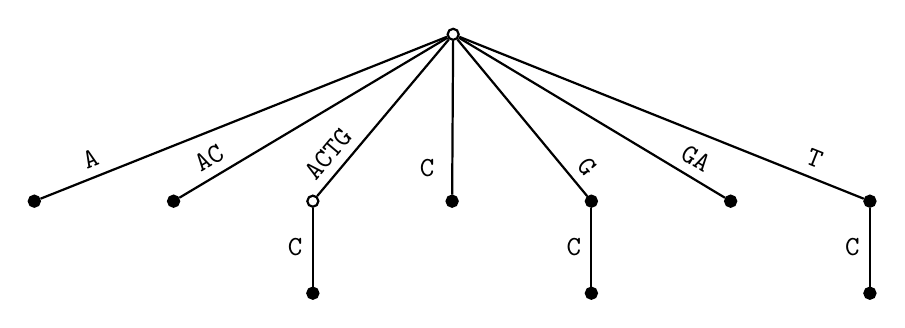
\begin{tikzpicture}[-,>=stealth',auto=false, thick,
    every label/.style={rectangle, font=\scriptsize, inner sep=3pt},
    	main node/.style={draw=black, fill=black, circle, inner sep=0pt, minimum size=4pt},
      	terminal/.style={circle,fill=white, inner sep=0.2pt}]

      \node[main node, fill=white] (root) [] {};
      \node[main node] (1) [below left=2cm and 5.2cm of root] {};
      \node[main node] (2) [right=1.6cm of 1] {};
      \node[main node, fill=white] (3) [right=1.6cm of 2] {};
      \node[main node] (4) [right=1.6cm of 3] {};
      \node[main node] (5) [right=1.6cm of 4] {};
      \node[main node] (6) [right=1.6cm of 5] {};
      \node[main node] (7) [right=1.6cm of 6] {};
      \node[main node] (31) [below=1cm of 3] {};
      %\node[main node] (41) [below=1cm of 4] {};
      \node[main node] (51) [below=1cm of 5] {};
      \node[main node] (71) [below=1cm of 7] {};

      \path[] (root) edge [] node [sloped, left=2cm, above] {\texttt{A}} (1);
      \path[] (root) edge [] node [sloped, left=1.4cm, above] {\texttt{AC}} (2);
      \path[] (root) edge [] node [sloped, left=0.8cm, above] {\texttt{ACTG}} (3);
      \path[] (root) edge [] node [left, below left=0.4cm and 0.1cm] {\texttt{C}} (4);
      \path[] (root) edge [] node [sloped, right=1cm, above] {\texttt{G}} (5);
      \path[] (root) edge [] node [sloped, right=1.4cm, above] {\texttt{GA}} (6);
      \path[] (root) edge [] node [sloped, right=2cm, above] {\texttt{T}} (7);
      \path[] (3) edge [] node [left] {\texttt{C}} (31);
      %\path[] (4) edge [] node [left] {\texttt{G}} (41);
      \path[] (5) edge [] node [left] {\texttt{C}} (51);
      \path[] (7) edge [] node [left] {\texttt{C}} (71);
    \end{tikzpicture}
    \caption{Motif trie for Example 1. The black nodes are maximal motifs (with their occurrence lists shown in Figure \ref{ex:one}(b))}
\end{figure}


\subsection{Motif Tries}
\label{sec:motiftrie}
%
We now exploit the machinery on alphabets described in Section~\ref{sub:efficient-representatin-motifs}. For the input sequence~$S$, consider the family $M_{qk}$ defined in Section~\ref{sec:preliminaries}, where each $m$ is seen as a string $m = m[1,\ell]$ of $\ell \leq k+1$ integers from~$1$ to~$|\salph|$. Although each $m$ can contain $O(n)$ symbols from $\calph$, we get a benefit from treating $m$ as a short string over $\salph$: unless specified otherwise, the prefixes and suffixes of $m$ are respectively $m[1,i]$ and $m[i,\ell]$ for $1\leq i \leq \ell$, where $\ell = \numdc(m) + 1 \leq k+1$. This helps with the following definition as it does not depend on the $O(n)$ symbols from $\calph$ in a maximal motif $m$ but it solely depends on its $\leq k+1$ length over~$\salph$.

\begin{definition}[Motif Trie]
A \emph{motif trie} $T$ is a trie over alphabet $\salph$ which stores all maximal motifs $\maxset \subseteq M_{qk}$ and their suffixes.
\end{definition}

As a consequence of being a trie, $T$ implicitly stores all prefixes of all the maximal motifs and edges in $T$ are labeled using characters from $\salph$.
Hence, all sub-motifs of the maximal motifs are stored in $T$, and the motif trie can be essentially seen as a generalized suffix trie\footnote{As it will be clear later, a compacted motif trie does not give any advantage in terms of the output-sensitive bound compared to the motif trie.} storing $\maxset$ over the alphabet $\salph$. From the definition, $T$ has 
%With $T$ being a trie, we inherit a number of useful properties. The number of leaves is 
$O((k+1) \cdot \nummax)$ leaves, the total number of nodes is $O(|T|) = O((k+1)^2 \cdot \nummax)$, and the height is at most $k+1$. 

We may consider a node $u$ in $T$ as a string generated over $\salph$ by spelling out the $\leq k+1$ integers from the root on the path towards $u$. To decode the motif stored in $u$, we retrieve these integers in $\salph$ and, using the suffix tree of $S$, we obtain the corresponding solid blocks over $\calph$ and insert a don't care symbol between every pair of consecutive solid blocks. When it is clear from the context, we will use $u$ to refer to \emph{(1)}~the node $u$ or \emph{(2)}~the string of integers from $\Pi$ stored in $u$, or \emph{(3)}~the corresponding motif from $(\calph \cup \{ \dontcare \})^*$. We reserve the notation $|u|$ to denote the length of motif $u$ as the number of characters from $\calph \cup \{ \dontcare \}$. Each node $u \in T$ stores a list $\occs{u}$ of occurrences of motif $u$ in $S$, i.e. $u$ occurs at $p$ in $S$ for $p \in \occs{u}$.

Since child edges for $u \in T$ are labeled with solid blocks, the child edge labels may be prefixes of each other, and one of the labels may be the empty string $\epsilon$ (which corresponds to having two neighboring don't cares in the decoded motif).


% HOW TO USE TRIE T, ASSUMING WE CAN GENERATE IT
\subsection{Reporting Maximal Motifs using Motif Tries}
\label{subec:reporting-maximal-motifs}
%
Suppose we are given a motif trie $T$ but we do not know which nodes of $T$ store the maximal motifs in $S$. We can identify and report the maximal motifs in $T$ in $O(|T|) = O((k+1)^2 \cdot \nummax) = O((k+1)^2 \cdot \sum_{m \in \maxset} \occ(m))$ time as follows.

We first identify the set $R$ of nodes $u \in T$ that are right-maximal motifs. A characterization of right-maximal motifs in $T$ is relatively simple: we choose a node $u \in T$ if \emph{(i)}~its parent edge label is not $\epsilon$, and \emph{(ii)}~$u$ has no descendant $v$ with a non-empty parent edge label such that~$|\occs{u}| = |\occs{v}|$. By performing a bottom-up traversal of nodes in $T$, computing for each node the length of the longest list of occurrences for a node in its subtree with a non-empty edge label, it is easy to find $R$ in time $O(|T|)$ and by Fact \ref{fact:right-maximal-suffix}, $|R| = O((k+1) \cdot \nummax)$.

Next we perform a radix sort on the set of pairs $\langle |\occs{u}|, \reverse(u) \rangle$, where $u \in R$ and $\reverse(u)$ denotes the reverse of the string $u$, to select the motifs that are also left-maximal (and thus are maximal). In this way, the suffixes of the maximal motifs become prefixes of the reversed maximal motifs. By Lemma~\ref{lemma:grouping}, those motifs sharing common prefixes are grouped together consecutively. However, there is a caveat, as one maximal motif $m'$ could be a suffix of another maximal motif $m$ and we do not want to drop~$m'$: in that case, we have that $|\occs{m}| \neq |\occs{m'}|$ by the definition of maximality. Hence, after sorting, we consider consecutive pairs $\langle |\occs{u_1}|, \reverse(u_1) \rangle$ and $\langle |\occs{u_2}|, \reverse(u_2) \rangle$ in the order, and eliminate $u_1$ iff $|\occs{u_1}|=|\occs{u_2}|$ and $u_1$ is a suffix of $u_2$ in time $O(k+1)$ per pair (i.e. prefix under $\reverse$). The remaining motifs are maximal.


\section{Building Motif Tries}
\label{sec:construction}

The goal of this section is to show how to efficiently build the motif trie $T$ discussed in Section~\ref{sec:motiftrie}. Suppose without loss of generality that enough new symbols are prepended and appended to the sequence $S$ to avoid border cases. We want to store the maximal motifs of $S$ in $T$ as strings of length $\leq k+1$  over $\salph$. Some difficulties arise as we do not know in advance which are the maximal motifs. Actually, we plan to find them \emph{during} the output-sensitive construction of $T$, which means that we would like to obtain a construction bound close to the term $\sum_{m \in \maxset} \! \occ(m)$ stated in Theorem~\ref{the:main}. 

We proceed in top-down and level-wise fashion by employing an \emph{oracle} that is invoked on each node~$u$ on the last level of the partially built trie, and which reveals the future children of $u$. The oracle is executed many times to generate~$T$ level-wise starting from its root~$u$ with $\occs{u} = \{1,\dots, n\}$, and stopping at level $k+1$ or earlier for each root-to-node path. 
Interestingly, this sounds like the wrong way to do anything efficiently, e.g. it is a slow way to build a suffix tree, however the oracle allows us to amortize the total cost to construct the trie. In particular, we can bound the total cost by the total number of occurrences of the maximal motifs stored in the motif trie. 
%with our oracle idea as we show in the following. 

%\begin{description}
%\item[(a)] The intermediate steps should avoid generating the motifs in $M_{qk} \setminus \maxset$ that are not suffixes of maximal motifs nor their prefixes, otherwise we cannot guarantee output-sensitive bounds as $M_{qk}$ can be exponentially larger than $\maxset$.
%\item[(b)] The construction cost charged to each node $u$ should be bounded by $O( \srt(\occs{u}) + (k+1) \cdot |\occs{u}|)$, where $\srt(\occs{u})$ is the cost of radix sorting for the list of occurrences $\occs{u}$. %(We prove and motivate this in Section~\ref{sec:bounding-construction-cost-motif-trie}.) 
%\item[(c)] The construction cost charged to each motif in the trie should be given in terms of its $\leq k+1$ length in $\salph$ rather than its $\leq n-1$ length in $\calph \cup \{ \dontcare \}$.
%\end{description}

The oracle is implemented by the $\generate{u}$ procedure that generates the children $u_1, \ldots, u_d$ of $u$. We ensure that \emph{(i)}~$\generate{u}$ operates on the $\leq k+1$ length motifs from $\salph$, and \emph{(ii)}~$\generate{u}$ avoids generating the motifs in $M_{qk} \setminus \maxset$ that are not suffixes or prefixes of maximal motifs. This is crucial, as otherwise we cannot guarantee output-sensitive bounds because $M_{qk}$ can be exponentially larger than $\maxset$.

In Section~\ref{sec:generate} we will show how to implement $\generate{u}$ and  prove:
%The time spent executing $\generate{u}$ is given by the following lemma, .

\begin{lemma}
  \label{lemma:generate_time}
  Algorithm $\generate{u}$ produces the children of $u$ and can be implemented in time $O(\srt(\occs{u}) + (k+1) \cdot |\occs{u}| + \sum_{i=1}^d |\occs{u_i}|)$. 
\end{lemma}


% BOUNDING THE SIZE OF T
%\subsection{Bounding the Total Construction Cost of Motif Tries}
%\label{sec:bounding-construction-cost-motif-trie}
%
By summing the cost to execute procedure $\generate{u}$ for all nodes $u \in T$, we now bound the construction time of $T$. Observe that when summing over $T$ the formula stated in Lemma~\ref{lemma:generate_time}, each node exists once in the first two terms and once in the third term, so the latter can be ignored when summing over $T$ (as it is dominated by the other terms)
\[
\sum_{u \in T} (\srt(\occs{u}) + (k+1) \cdot |\occs{u}| + \sum_{i=1}^d |\occs{u_i}|) = O\left(\sum_{u \in   T} (\srt(\occs{u}) + (k+1) \cdot |\occs{u}|) \right) ~~ .
\]

% = O(n(k+1) + (k+1) \times \sum_{u \in T} |\occs{u}|))$, where 
\noindent We bound 
\[
\sum_{u \in T} \srt(\occs{u}) = O\left( n(k+1) + \sum_{u \in T} |\occs{u}|\right)
\] 
by running a single cumulative radix sort for all the instances over the several nodes $u$ at the same level, allowing us to amortize the additive cost $O(n)$ of the radix sorting among nodes at the same level (and there are at most $k+1$ such levels).

To bound $\sum_{u \in T} |\occs{u}|$, we observe $\sum_i |\occs{u_i}| \geq |\occs{u}|$ (as trivially the $\epsilon$ extension always maintains the number of occurrences of its parent). Consequently we can charge each leaf $u$ the cost of its $\leq k$ ancestors, so \[
\sum_{u \in T} |\occs{u}| = O\left((k+1) \times \sum_{\mathrm{leaf\ }u \in T} |\occs{u}|\right) ~~ .
\]

Finally, from Section~\ref{sec:motiftrie} there cannot be more leaves than maximal motifs in $\maxset$ and their suffixes, and the occurrence lists of maximal motifs dominate the size of the non-maximal ones in $T$, which allows us to bound: 
\[
(k+1) \times \sum_{\mathrm{leaf\ }u \in T} |\occs{u}| = O\left((k+1)^2 \times \sum_{m \in \maxset} \occ(m)\right) ~~ .
\]   
Adding the $O(n \log \calph)$ cost for the suffix tree and the LCA ancestor data structure of Section~\ref{sub:efficient-representatin-motifs}, we obtain:

\begin{theorem}\label{the:trie}
    Given a sequence $S$ of $n$ objects over an alphabet $\calph$ and two integers $q > 1$ and $k \geq 0$, a motif trie containing the maximal motifs $\maxset \subseteq M_{qk}$ and their occurrences $\occ(m)$ in $S$ for $m \in \maxset$  can be built in time and space
$O \Bigl( n (k + \log \calph) + (k+1)^3 \times \sum_{m \in \maxset} \occ(m) \Bigr)$.
\end{theorem}


\section{Implementing $\generate{u}$}\label{sec:generate}
We now show how to implement $\generate{u}$ in the time bounds stated by Lemma~\ref{lemma:generate_time}. The idea is as follows. We first obtain $\sortoccs{u}$, which is an array storing the occurrences in $\occs{u}$, sorted lexicographically according to the suffix associated with each occurrence. We can then show that there is a bijection between the children of $u$ and a set of maximal intervals in $\sortoccs{u}$. By exploiting the properties of these intervals, we are able to find them efficiently through a number of scans of $\sortoccs{u}$. The bijection implies that we thus efficiently obtain the new children of $u$.


\subsection{Nodes of the Motif Trie as Maximal Intervals}
\label{sub:intervals}
The key point in the efficient implementation of the oracle $\generate{u}$ is to relate each node $u$ and its future children $u_1, \ldots, u_d$ labeled by solid blocks $b_1, \ldots, b_d$, respectively, to some suitable intervals that represent their occurrence lists $\occs{u}, \occs{u_1}, \ldots, \occs{u_d}$. 
Though the idea of using intervals for representing trie nodes is not new (e.g. in \cite{abouelhoda2004replacing}), we use intervals to expand the trie rather than merely representing its nodes. Not all intervals generate children as not all solid blocks that extend $u$ necessarily generate a child. Also, some of the solid blocks $b_1, \ldots, b_d$ can be prefixes of each other and one of the intervals can be the empty string $\epsilon$. To select them carefully, we need some definitions and properties.

\subparagraph*{Extensions.}
%
For a position $p \in \occs{u}$, we define its \emph{extension} as the suffix $\ext(p, u) = S[p + |u| + 1, n]$ that starts at the position after $p$ with an offset equivalent to skipping the prefix matching $u$ plus one symbol (for the don't care). We may write $\ext(p)$, omitting the motif $u$ if it is clear from the context. We also say that the \emph{skipped characters} $\skipchar(p)$ at position $p \in \occs{u}$ are the $d=\numdc(u)+2$ characters in $S$ that specialize $u$ into its occurrence $p$: formally,  $\skipchar(p) = \langle c_0, c_1, \ldots, c_{d-1}  \rangle$ where $c_0 = S[p-1]$, $c_{d-1} = S[p+|u|]$, and $c_i = S[p+j_i-1]$, for $1 \leq i \leq d-2$, where $u[j_i] = \dontcare$ is the $i$th don't care in $u$. 

We denote by $\sortoccs{u}$ the list $\occs{u}$ sorted using as keys the integers for $\ext(p)$ where $p \in \occs{u}$. (We recall from Section~\ref{sub:efficient-representatin-motifs} that the suffixes are represented in the alphabet~$\salph$, and thus $\ext(p)$ can be seen as an integer in $\salph$.) By Lemma~\ref{lemma:grouping} consecutive positions in $\sortoccs{u}$ share common prefixes of their extensions. Lemma~\ref{lem:commonPref} below states that these prefixes are the candidates for being correct edge labels for expanding $u$ in the trie. 
\begin{lemma}
  \label{lem:commonPref}
    Let $u_i$ be a child of node $u$, $b_i$ be the label of  edge $(u, u_i)$, and $p \in \occs{u}$ be an occurrence position. If position $p \in \occs{u_i}$ then $b_i$ is a prefix of $\ext(p, u)$.
\end{lemma}
\begin{proof}
    Assume otherwise, so $p \in \occs{u} \cap \occs{u_i}$ but $b_i \not \in \prefset(\ext(p, u))$. 
    Then there is a mismatch of solid block $b_i$ in $\ext(p, u)$, since at least one of the characters in $b_i$ is not in $\ext(p, u)$. But this means that $u_i$ cannot occur at position $p$, and consequently $p \not \in \occs{u_i}$, which is a contradiction.
\end{proof}

\subparagraph*{Intervals.}
%
Lemma~\ref{lem:commonPref} states a necessary condition, so we have to filter the candidate prefixes of the extensions. We use the following notion of intervals to facilitate this task. We call $\interval{} \subseteq \sortoccs{u}$ an \emph{interval} of $\sortoccs{u}$ if $\interval{}$ contains consecutive entries of $\sortoccs{u}$. We write $\interval{} = [i, j]$ if $\interval{}$ covers the range of indices from $i$ to $j$ in $\sortoccs{u}$. 
The \emph{longest common prefix} of an interval is defined as $\ilcp(\interval{}) = \min_{p_1, p_2 \in \interval{}} \lcp(\ext(p_1), \ext(p_2))$, which is a solid block in $\salph$ as discussed at the end of Section~\ref{sub:efficient-representatin-motifs}. By Lemma~\ref{lemma:grouping}, $\ilcp(\interval{}) = \lcp(\ext(\sortoccs{u}[i]), \ext(\sortoccs{u}[j]))$ can be computed in $O(1)$ time, where $\sortoccs{u}[i]$ is the first and $\sortoccs{u}[j]$ the last element in $\interval{} = [i, j]$. 

\subparagraph*{Maximal Intervals.}
%
An interval $\interval{} \subseteq \sortoccs{u}$ is \emph{maximal} if \emph{(1)}~there are at least~$q$ positions in $\interval{}$ (i.e. $|\interval{}| \geq q$), \emph{(2)}~motif $u$ cannot be specialized with the skipped characters in $\skipchar(p)$ where $p \in \interval{}$, and \emph{(3)}~any other interval $\interval{}' \subseteq \sortoccs{u}$ that strictly contains $\interval{}$ has a shorter common prefix (i.e. $|\ilcp(\interval{}')| < |\ilcp(\interval{})|$ for $\interval{}' \supset \interval{}$) \footnote{%
%While conditions~\emph{(1)} and~\emph{(3)} are intuitive, as we want the largest intervals with $\geq q$ positions that cannot be extended, condition~\emph{(2)} is less intuitive but has a dramatic effect on the complexity. To see why consider an interval $\interval{}$ that satisfies~\emph{(1)} and~\emph{(3)} but not~\emph{(2)}. This means that the occurrences of $u$ in $S$ restricted at positions $p \in \interval{}$ have the same symbol in correspondence of the same $\dontcare$ in $u$ (while this is not true for all $p \in \sortoccs{u}$). 
%In the full version we show that c
Condition~\emph{(2)} is needed to avoid the enumeration of either motifs from $M_{qk} \setminus \maxset$ or duplicates from $\maxset$.}.
We denote by $\intervalset{u}$ the \emph{set of all maximal intervals} of $\sortoccs{u}$, and show that $\intervalset{u}$ form a tree covering of $\sortoccs{u}$. A similar lemma for intervals over the LCP array of a suffix tree was given in \cite{abouelhoda2004replacing}.
\begin{lemma}
  \label{lem:intOverlap}
    Let $\interval{1}, \interval{2} \in \intervalset{u}$ be two maximal intervals, where $\interval{1} \not = \interval{2}$ and $|\interval{1}| \leq  |\interval{2}|$.
    Then either $\interval{1}$ is contained in $\interval{2}$ with a longer common prefix (i.e. $\interval{1} \subset \interval{2}$ and $|\ilcp(\interval{1})| > |\ilcp(\interval{2})|$) or the intervals are disjoint (i.e. $\interval{1} \cap \interval{2} = \emptyset$). 
\end{lemma}
\begin{proof}
    Let $\interval{1} = [i, j]$ and $\interval{2} = [i', j']$. 
    %Since $\interval{1} \not = \interval{2}$, either $i < i'$ or $j > j'$. 
    Assume partial overlaps are possible, $i' \leq i \leq j' < j$, to obtain a contradiction.
    Since $|\ilcp(\interval{1})| \geq |\ilcp(\interval{2})|$, the interval $\interval{3} = [j', j]$ has a longest common prefix $|\ilcp(\interval{3})| \geq |\ilcp(\interval{2})|$, and so $\interval{2}$ could have been extended and was not maximal, giving a contradiction. 
    The remaining cases are symmetric.
\end{proof}

The next lemma establishes a useful bijection between maximal intervals $\intervalset{u}$ and children of $u$, motivating why we use intervals to expand the motif trie. 
\begin{lemma}
  \label{lem:bijection}
    Let $u_i$ be a child of a node $u$. Then the occurrence list $\occs{u_i}$ is a permutation of a maximal interval $\interval{} \subseteq \intervalset{u}$, and vice versa. The label on edge $(u, u_i)$ is the solid block $b_i = \ilcp(\interval{})$. No other children or maximal intervals have this property with $u_i$ or $\interval{}$.
\end{lemma}
\begin{proof}
    We prove the statement by assuming that $T$ has been built, and that the maximal intervals have been computed for a node $u \in T$.

    We first show that given a maximal interval $\interval{} \in \intervalset{u}$, there is a single corresponding child $u_i \in T$ of $u$.
    Let $b_i = \ilcp(\interval{})$ denote the longest common prefix of occurrences in $\interval{}$, and note that $b_i$ is distinct among the maximal intervals in $\intervalset{u}$. Also, since $b_i$ is a common prefix for all occurrence extensions in $\interval{}$, the motif $u \dontcare b_i$ occurs at all locations in $\interval{}$ (as we know that $u$ occurs at those locations). 
    Since $|\interval{}| \geq q$ and $u \dontcare b_i$ is an occurrence at all $p \in \interval{}$, there must be a child $u_i$ of $u$, where the edge $(u, u_i)$ is labeled $b_i$ and where $\interval{} \subseteq \occs{u_i}$. From the definition of tries, there is at most one such node. There can be no $p' \in \occs{u_i} - \interval{}$, since that would mean that an occurrence of $u \dontcare b_i$ was not stored in $\interval{}$, contradicting the maximality assumption of $\interval{}$. Finally, because $|\skipset{\interval{}}| \geq 2$ and $b_i$ is the longest common prefix of all occurrences in $\interval{}$, not all occurrences of $u_i$ can be extended to the left using one symbol from $\calph$. Thus, $u_i$ is a prefix or suffix of a maximal motif.
    
    We now prove the other direction, that given a child $u_i \in T$ of $u$, we can find a single maximal interval $\interval{} \in \intervalset{u}$.    
    First, denote by $b_i$ the label on the $(u, u_i)$ edge. From Lemma \ref{lem:commonPref}, $b_i$ is a common prefix of all extensions of the occurrences in $\sortoccs{u_i}$. Since not all occurrences of $u_i$ can be extended to the left using a single symbol from $\calph$, $b_i$ is the longest common prefix satisfying this, and there are at least two different skipped characters of the occurrences in $\occs{u_i}$. 
    Now, we know that $u_i = u \dontcare b_i$ occurs at all locations $p \in \occs{u_i}$. Observe that $\occs{u_i}$ is a (jumbled) interval of $\sortoccs{u}$ (since otherwise, there would be an element $p' \in \sortoccs{u}$ which did not match $u_i$ but had occurrences from $\occs{u_i}$ on both sides in $\sortoccs{u}$, contradicting the grouping of $\sortoccs{u}$). All occurrences of $u_i$ are in $\occs{u_i}$ so $\occs{u_i}$ is a (jumbled) maximal interval of $\sortoccs{u}$.
    We just described a maximal interval with a distinct set of occurrences, at least two different skipped characters and a common prefix, so there must surely be a corresponding interval $\interval{} \in \intervalset{u}$ such that $\ilcp(\interval{}) = b_i$, $|\skipset{\interval{}}| \geq 2$ and $\occs{u_i} \subseteq \interval{}$. There can be no $p' \in \interval{} - \occs{u_i}$, as $p' \in \occs{u}$ and $b_i \in \prefset(\ext(p', u))$ means that $p' \in \occs{u_i}$.
\end{proof}


\subsection{Exploiting the Properties of Maximal Intervals}
%
We now use the properties shown above to implement the oracle $\generate{u}$, resulting in Lemma~\ref{lemma:generate_time}. Observe that the task of $\generate{u}$ can be equivalently seen by Lemma~\ref{lem:bijection} as the task of finding all maximal intervals $\intervalset{u}$ in $\sortoccs{u}$, where each interval $\interval{} \in \intervalset{u}$ corresponds exactly to a distinct child $u_i$ of $u$. We describe three main steps, where the first takes $O(\srt(\occs{u}) + (k+1) \cdot |\occs{u}| )$ time, and the others require $O(\sum_{i=1}^d |\occs{u_i}|)$ time. The interval $\interval{} = \sortoccs{u}$ corresponding to the solid block~$\epsilon$ is trivial to find, so we focus on the rest. We assume $\numdc(u) < k$, as otherwise we are already done with $u$.


\subparagraph*{Step~1. Sort occurrences and find maximal runs of skipped characters.} 
%
We perform a radix-sort of $\occs{u}$ using the extensions as keys, seen as integers from $\salph$, thus obtaining array $\sortoccs{u}$. To facilitate the task of checking condition~\emph{(2)} for the maximality of intervals, we compute for each index $i \in \sortoccs{u}$ 
%at index $i(p)$ in $\sortoccs{u}$  
the smallest index $R(i) > i$ in $\sortoccs{u}$ such that motif $u$ cannot be specialized with the skipped characters in $\skipchar(\sortoccs{u}[j])$ where $j \in [i, R(i)]$. That is, there are at least two different characters from $\calph$ hidden by each of the skipped characters in the interval. (If $R(i)$ does not exist, we do not create $[i, R(i)]$.)
We define $|\skipset{\interval{}}|$ as the minimum number of different characters covered by each skipped character in interval $\interval{}$, and note that $|\skipset{[i, R(i)]}| \geq 2$ by definition. 

To do so we first find, for each skipped character position, all indices where a maximal run of equal characters end: $R(i)$ is the maximum indices for the given $i$. This helps us because for any index $i$ inside such a block of equal characters, $R(i)$ must be on the right of where the block ends (otherwise $[i, R(i)]$ would cover only one character in that block). 
Using this to calculate $R(i)$ for all indices $i \in \sortoccs{u}$ from left to right, we find each answer in time $O(k+1)$, and $O((k+1) \cdot |\sortoccs{u}|)$ total time. We denote by $\rintset$ the set of intervals $[i, R(i)]$ for $i \in \sortoccs{u}$. 

\begin{lemma}
  \label{lemma:R-prefix}
  For any maximal interval $\interval{} \equiv [i,j] \in \intervalset{u}$, there exists $R(i) \leq j$, and thus $[i,R(i)]$ is an initial portion of $\interval{}$.
\end{lemma}

\subparagraph*{Step~2. Find maximal intervals with handles.}
%

We want to find all maximal intervals covering each position of $\sortoccs{u}$. To this end, we introduce \emph{handles}. 
For each $p \in \sortoccs{u}$, its \emph{interval domain} $D(p)$ is the set of intervals $\interval{}' \subset \sortoccs{u}$ such that $p \in \interval{}'$ and $|\skipset{\interval{}'}| \geq 2$.
We let $\maxlcp{p}$ be the length of the longest shared solid block prefix $b_i$ over $D(p)$, namely, $\maxlcp{p} = \max_{\interval{}' \in D(p)} |\ilcp(\interval{}')|$. For a maximal interval $\interval{} \subseteq \intervalset{u}$, if $|\ilcp(\interval{})| = \maxlcp{p}$ for some $p \in \interval{}$ we call $p$ a \emph{handle} on $\interval{}$. Handles are relevant for the following reason.

\begin{lemma}
  \label{lem:handles}
    For each maximal interval $\interval{} \subseteq \intervalset{u}$, either there is a handle $p \in \sortoccs{u}$ on $\interval{}$, or $\interval{}$ is fully covered by $\geq 2$ adjacent maximal intervals with handles.
\end{lemma}
\begin{proof}
    From Lemma \ref{lem:intOverlap}, any maximal interval $\interval{} \in \intervalset{u}$ is either fully contained in some other maximal interval, or completely disjoint from other maximal intervals. Partial overlaps of maximal intervals are impossible.
    
    Now, assume there is no handle $p \in \occs{u}$ on $\interval{}$. If so, all $p' \in \interval{}$ has $\maxlcp{p'} \not = |\ilcp(\interval{})|$ (since otherwise $p' \in \interval{}$ and $\maxlcp{p'} = |\ilcp(\interval{})|$ and thus $p'$ was a handle on $\interval{}$).
    Clearly for all $p' \in \interval{}$, $|\ilcp(\interval{})|$ is a lower bound for $\maxlcp{p'}$. Thus, to get a contradiction it must be the case that $\maxlcp{p'} > |\ilcp(\interval{})|$ for all $p' \in \interval{}$.
    This can only happen if $\interval{}$ is completely covered by $\geq 2$ maximal intervals with a larger longest common prefix. From Lemma \ref{lem:intOverlap}, a single interval $\interval{}'$ is not enough because $\interval{}'$ is fully contained (or completely disjoint) in $\interval{}$ if $|\ilcp(\interval{}')| \geq |\ilcp(\interval{})|$.
\end{proof}

Let $\handlevalset{u}$ denote the set of maximal intervals with handles. We now show how to find the set $\handlevalset{u}$ among the intervals of $\sortoccs{u}$. Observe that for each occurrence $p \in \sortoccs{u}$, we must find the interval $\interval{}'$ with the largest $\ilcp(\interval{}')$ value among all intervals containing~$p$.

From the definition, a handle on a maximal interval $\interval{}'$ requires $|\skipset{\interval{}'}| \geq 2$, which is exactly what the intervals in $\rintset$ satisfy. As the $\ilcp$ value can only drop when extending an interval, these are the only candidates for maximal intervals with handles. Note that from Lemma \ref{lemma:R-prefix}, $\rintset$ contains a prefix for all of the (not expanded) maximal intervals because it has all intervals from left to right obeying the conditions on length and skipped character conditions. Furthermore, $|\rintset| = O(|\sortoccs{u}|)$, since only one $R(i)$ is calculated for each starting position. Among the intervals $[i, R(i)] \in \rintset$, we will now show how to find those with maximum $\ilcp$ (i.e. where the $\ilcp$ value equals $\maxlcp{p}$) for all $p$.

%To avoid using a priority queue to find $\maxlcp{p}$ as the maximum over the intervals in $\rintset$, which would require super-linear time, 
We use an idea similar to that used in Section \ref{subec:reporting-maximal-motifs} to filter maximal motifs from the right-maximal motifs. 
We sort the intervals $\interval{}' = [i, R(i)] \in \rintset$ in decreasing lexicographic order according to the pairs
%$\langle|\ilcp(\interval{}')|, R(i), i\rangle$. 
$\langle|\ilcp(\interval{}')|, -i\rangle$ (i.e. decreasing $\ilcp$ values but increasing indices $i$), to obtain the sequence $\candset$. 
Thus, if considering the intervals left to right in $\candset$, we consider intervals with larger $\ilcp$ values from left to right in $S$ before moving to smaller $\ilcp$ values. 
%For each of the interval in this ordering, we check if it is a new maximal interval with a handle. If so, we expand the interval until the the $\ilcp$ value changes and mark the newly covered occurrences in $\sortoccs{u}$. %This is done by first filtering $\rintset$ and afterwards using a number of linear scans to produce the final set of maximal intervals with handles $\handlevalset{u}$.


%We scan the ordered intervals from left to right and compare intervals $\interval{1} = [i, R(i)], \interval{2} = [j, R(j)]$: we discard interval $\interval{1}$ if $|\ilcp(\interval{1})| = |\ilcp(\interval{2})|$, $R(i) = R(j)$ and $i > j$ (as $\interval{1}$ is fully contained in $\interval{2}$ with the same $\ilcp$ value, $\interval{1}$ cannot be maximal). 

%After elimination, we scan the remaining ordered intervals from left to right and compare intervals $\interval{1} = [i, R(i)], \interval{2} = [j, R(j)]$: we merge intervals $\interval{1}$ and $\interval{2}$ into $\interval{3} = [i, R(j)]$ if $|\ilcp(\interval{1})| = |\ilcp(\interval{2})|$, $R(j) > R(i)$ and $R(i) \geq j > i$ (since the intervals are overlapping with the same $\ilcp$ value). After the merge procedure, each $p \in \sortoccs{u}$ only has a single maximal interval candidate remaining in the set, which we call the candidate set $\candset$. Observe that the set may contain intervals that overlap and which are not maximal. 

%We will now show how to find $\handlevalset{u}$ by processing $\candset$ to find the maximal intervals with handles. $\candset$ is considered from left to right using the ordering previously described. 
Consider an interval $\interval{p} = [i, R(i)] \in \candset$. The idea is that we determine if $\interval{p}$ has already been added to $\handlevalset{u}$ by some previously processed handled maximal interval. If not, we expand the interval (making it maximal) and add it to $\handlevalset{u}$, otherwise $\interval{p}$ is discarded. When $\candset$ is fully processed, all occurrences in $\sortoccs{u}$ are covered by maximal intervals with handles.

First, since maximal intervals must be fully contained in each other (from Lemma \ref{lem:intOverlap}), we determine if $\interval{p} = [i, R(i)] \in \candset$ is already fully covered by previously expanded intervals (with larger $\ilcp$ values) -- if not, we must expand $\interval{p}$. Clearly, if either $i$ or $R(i)$ is not included in any previous expansions, we must expand $\interval{p}$. Otherwise, if both $i$ and $R(i)$ is part of a single previous expansion $\interval{q} \in \candset$, $\interval{p}$ should not be expanded. If $i$ and $R(i)$ is part of two different expansions $\interval{q}$ and $\interval{r}$ we compare their extent values: $\interval{p}$ must be expanded if some $p \in \interval{p}$ is not covered by either $\interval{q}$ or $\interval{r}$. To enable these checks we mark each $j \in \sortoccs{u}$ with the longest processed interval that contains it (during the expansion procedure below).

Secondly, to expand $\interval{p}$ maximally to the left and right, we use pairwise $\lcp$ queries on the border of the interval. Let $a \in \interval{p}$ be a border occurrence and $b \not \in \interval{p}$ be its neighboring occurrence in $\sortoccs{u}$ (if any, otherwise it is trivial). When $|\lcp(a, b)| < |\ilcp(\interval{p})|$, the interval cannot be expanded to span $b$. When the expansion is completed, $\interval{p}$ is a maximal interval and added to $\handlevalset{u}$. As previously stated, all elements in $\interval{p}$ are marked as being part of their longest covering handled maximal interval by writing $\interval{p}$ on each of its occurrences.

\subparagraph*{Step~3. Find composite maximal intervals covered by maximal intervals with handles.}
%
From Lemma \ref{lem:handles}, the only remaining type of intervals are composed of maximal intervals with handles from the set $\handlevalset{u}$. A \emph{composite maximal interval} must be the union of a sequence of adjacent maximal intervals with handles. We find these as follows. We order $\handlevalset{u}$ according to the starting position and process it from left to right in a greedy fashion, letting $\interval{h} \in \handlevalset{u}$ be one of the previously found maximal intervals with handles. Each interval $\interval{h}$ is responsible for generating exactly the composite maximal intervals where the sequence of covering intervals starts with $\interval{h}$ (and which contains a number of adjacent intervals on the right). Let $\interval{h}' \in \handlevalset{u}$ be the interval adjacent on the right to $\interval{h}$, and create the composed interval $\interval{c} = \interval{h} + \interval{h}'$ (where $+$ indicates the concatenation of consecutive intervals). To ensure that a composite interval is new, we check as in Step 2 that there is no previously generated maximal interval $\interval{}$ with $|\ilcp(\interval{})| = |\ilcp(\interval{c})|$ such that $\interval{c} \subseteq \interval{}$. This is correct since if there is such an interval, it has already been fully expanded by a previous expansion (of composite intervals or a handled interval). Furthermore, if there is such an interval, all intervals containing $\interval{c}$ with shorter longest common prefixes have been taken care of, since from Lemma \ref{lem:intOverlap} maximal intervals cannot straddle each other. If $\interval{c}$ is new, we know that we have a new maximal composite interval and can continue expanding it with adjacent intervals. If the length of the longest common prefix of the expanded interval changes, we must perform the previous check again (and add the previously expanded composite interval to $\intervalset{u}$).

\vspace{1em}
By analyzing the algorithm described, one can prove the following two lemmas showing that the motif trie is generated correctly. While Lemma \ref{lem:soundness} states that $\epsilon$-extensions may be generated (i.e. a sequence of $\dontcare$ symbols may be added to suffixes of maximal motifs), a simple bottom-up cleanup traversal of $T$ is enough to remove these.

\begin{lemma}\label{lem:soundness}
\textbf{(Soundness)} Each motif stored in $T$ is a prefix or an $\epsilon$-extension of some suffix of a maximal motif (encoded using alphabet $\salph$ and stored in $T$).
\end{lemma}
\begin{proof}
    The property to be shown for motif $m \in T$ is: \emph{(1)} $m$ is a prefix of some suffix of a maximal motif $m' \in \maxset$ (encoded using alphabet $\salph$), or \emph{(2)} $m$ is the suffix of some maximal motif $m' \in \maxset$ extended by at most $k$ $\epsilon$ solid blocks (and don't cares). 
    
    Note that we only need to show that $\generate{u}$ can only create children of $u \in T$ with the desired property. We prove this by induction. In the basis, $u$ is the root and $\generate{u}$ produce all motifs such that adding a character from $\calph$ to either end decreases the number of occurrences: this is ensured by requiring that there must be more than two different skipped characters in the occurrences considered, using the LCP of such intervals and only extending intervals to span occurrences maintaining  the same LCP length. Since there are no don't cares in these motifs they cannot be specialized and so each of them must be a prefix or suffix of some maximal motif.
    
    For the inductive step, we prove the property by construction, assuming $\numdc(u) < k$. Consider a child $u_i$ generated by $\generate{u}$ by extending with solid block $b_i$: it must not be the case that, without losing occurrences,
    \emph{(a)} $u_i$ can be specialized by converting one of its don't cares into a solid character from $\calph$, or
    \emph{(b)} $u_i$ can be extended in either direction using only characters from $\calph$.
    If either of these conditions is violated, $u_i$ can clearly not satisfy the property (in the first case, the generalization $u_i$ is not a suffix or prefix of the specialized maximal motif). However, these conditions are sufficient, as they ensure that $u_i$ is encoded using $\salph$ and cannot be specialized or extended without using don't cares. Thus, if $b_i \not = \epsilon$, $u_i$ is either a prefix of some suffix of a maximal motif (since $u_i$ ends with a solid block it may be maximal), or if $b_i = \epsilon$, $u_i$ may be an $\epsilon$-extension of $u$ (or a prefix of some suffix if some descendant of $u_i$ has the same number of occurrences and a non-$\epsilon$ parent edge).  
    
    By the induction hypothesis, $u$ satisfies \emph{(1)} or \emph{(2)} and $u$ is a prefix of $u_i$. Furthermore, the occurrences of $u$ have more than one different character at all locations covered by the don't cares in $u$ (otherwise one of those locations in $u$ could be specialized to the common character).     
    When generating children, we ensure that \emph{(a)} cannot occur by forcing the occurrence list of generated children to be large enough that at least two different characters is covered by each don't care. That is, $u_i$ may only be created if it cannot be specialized in any location, ensured by only considering intervals covering $L(p)$ and $R(p)$. Condition \emph{(b)} is avoided by ensuring that there are at least two different skipped characters for the occurrences of $u_i$ and forcing the extending block $b_i$ to be maximal under that condition. 
\end{proof}

\begin{lemma}\label{lem:completeness}
\textbf{(Completeness)} If $m \in \maxset$, $T$ stores $m$ and its suffixes.
\end{lemma}
\begin{proof}
    We summarize the proof that $\generate{u}$ is correct and the correct motif trie is produced. From Lemma \ref{lem:handles}, we create all intervals in $\generate{u}$ by expanding those with handles, and expanding all composite intervals from these. By Lemma \ref{lem:bijection} the intervals found correspond exactly to the children of $u$ in the motif trie. Thus, as $\generate{u}$ is executed for all $u \in T$ when $\numdc(u) \leq k-1$, all nodes in $T$ is created correctly until depth $k+1$. 
    
    Now clearly $T$ contains $\maxset$ and all the suffixes: for a maximal motif $m \in \maxset$, any suffix $m'$ is generated and stored in $T$ as \emph{(1)} $\occ(m') \geq \occ(m)$ and \emph{(2)} $\numdc(m') \leq \numdc(m)$. 
\end{proof}



%%%%%%%%%%%%%%%%%%%%%%%%%%%%%%%%%%%%%%%%%%%%%%%%%%%%%%%%%%%%%%%%%%
%%%%%%%%%%%%%%%%%%%%% REFERENCES, APPENDIX %%%%%%%%%%%%%%%%%%%%%%%
%%%%%%%%%%%%%%%%%%%%%%%%%%%%%%%%%%%%%%%%%%%%%%%%%%%%%%%%%%%%%%%%%%

%\textbf{History}
%This theoretical work was inspired by an algorithm implemented for motif extraction in DNA sequences, which performed very well. 
%The present paper is the result of explaining its behavior, improving it in many respects. 
 %text, algorithm, ds
%!TEX root = ../../../Thesis.tex


\chapter{Compressed Data Structures for Range Searching}


%%%%%%%%%%%%%%%%%%%%%%%%%%%%%%%%%%%%%%%%%%%%%%%%%%%%%%%%%%%%%%%%%%
%%%%%%%%%%%%%%%%%%%%%%%%%%% TITLEPAGE %%%%%%%%%%%%%%%%%%%%%%%%%%%%
%%%%%%%%%%%%%%%%%%%%%%%%%%%%%%%%%%%%%%%%%%%%%%%%%%%%%%%%%%%%%%%%%%
%\newcommand*\samethanks[1][\value{footnote}]{\footnotemark[#1]}

%\title{Compressed Data Structures\\for Range Searching\thanks{Supported by a grant from the Danish National Advanced Technology Foundation.}}
%\author{
%	Philip Bille\thanks{Supported by a grant from the Danish Council for Independent Research $\vert$ Natural Sciences.}
%	\and Inge Li G{\o}rtz\samethanks
% 	\and S{\o}ren Vind
%}
%\date{}
%\institute{DTU Compute, Technical University of Denmark, DK-2800 Kgs. Lyngby, Denmark \\ \email{$\{$phbi,inge,sovi$\}$@dtu.dk}}


%\begin{document}
%\pagestyle{plain}	
%\linenumbers

%\maketitle
%\setcounter{footnote}{0}

% Fix grants, reset footnote counter to arabic.
%\renewcommand{\thefootnote}{\fnsymbol{footnote}}
%\footnotetext[1]{Supported by a grant from the Danish National Advanced Technology Foundation.} %star
%\footnotetext[4]{Supported by a grant from the Danish Council for Independent Research $\vert$ Natural Sciences.} %dagger

%\renewcommand{\thefootnote}{\arabic{footnote}}

%%%%%%%%%%%%%%%%%%%%%%%%%%%%%%%%%%%%%%%%%%%%%%%%%%%%%%%%%%%%%%%%%%
%%%%%%%%%%%%%%%%%%%%%%%%%%% ABSTRACT %%%%%%%%%%%%%%%%%%%%%%%%%%%%%
%%%%%%%%%%%%%%%%%%%%%%%%%%%%%%%%%%%%%%%%%%%%%%%%%%%%%%%%%%%%%%%%%%
\begin{abstract}
We study the orthogonal range searching problem on points that have a significant number of \emph{geometric repetitions}, that is, subsets of points that are identical under translation. Such repetitions occur in scenarios such as image compression, GIS applications and in compactly representing sparse matrices and web graphs. Our contribution is twofold. 
First, we show how to compress geometric repetitions that may appear in standard range searching data structures (such as K-D trees, Quad trees, Range trees, R-trees, Priority R-trees, and K-D-B trees), and how to implement subsequent range queries on the compressed representation with only a constant factor overhead. 
Secondly, we present a compression scheme that efficiently identifies geometric repetitions in point sets, and produces a hierarchical clustering of the point sets, which combined with the first result leads to a compressed representation that supports range searching. 
\end{abstract}

%%%%%%%%%%%%%%%%%%%%%%%%%%%%%%%%%%%%%%%%%%%%%%%%%%%%%%%%%%%%%%%%%%
%%%%%%%%%%%%%%%%%%%%%%%%%% INTRODUCTION %%%%%%%%%%%%%%%%%%%%%%%%%%
%%%%%%%%%%%%%%%%%%%%%%%%%%%%%%%%%%%%%%%%%%%%%%%%%%%%%%%%%%%%%%%%%%
\section{Introduction}
The \emph{orthogonal range searching} problem is to store a set of axis-orthogonal $k$-dimensional objects to efficiently answer \emph{range queries}, such as reporting or counting all objects inside a $k$-dimensional query range. Range searching is a central primitive in a wide range of applications and has been studied extensively over the last 40 years~\cite{bentley1975multidimensional, bentley1979multidimensional, orenstein1982multidimensional, bentley1980decomposable, lueker1978data, lee1980quintary, guttman1984r, clarkson1983fast, kanth1999optimal, van1991dividedk, gaede1998multidimensional, bayer1972organization, arge2008priority, robinson1981kdb, procopiuc2003bkd, comer1979ubiquitous, eppstein2008skip} (Samet presents an overview in \cite{samet1990applications}). 

In this paper we study range searching on points that have a significant number of \emph{geometric repetitions}, that is, subsets of points that are identical under translation. Range searching on points sets with geometric repetitions arise naturally in several scenarios such as data and image analysis \cite{tetko2001pattern, pajarola2000image, dick2009a}, GIS applications \cite{schindler2008detecting, zhu2002efficient, haegler2010a, dick2009a}, and in compactly representing sparse matrices and web graphs~\cite{Galli98compressionof, brisaboa2009k2, brisaboaainterleaved, de2013compact}.

Our contribution is twofold. 
First, we present a simple technique to effectively compress geometric repetitions that may appear in standard range searching data structures (such as K-D trees, Quad trees, Range trees, R-trees, Priority R-trees, and K-D-B trees). Our technique replaces repetitions within the data structures by a single copy, while only incurring an $O(1)$ factor overhead in queries (both in standard RAM model and I/O model of computation). The key idea is to compress the underlying tree representation of the point set into a corresponding minimal DAG that captures the repetitions. We then show how to efficiently simulate range queries directly on this DAG. This construction is the first solution to take advantage of geometric repetitions. Compared to the original range searching data structure the time and space complexity of the compressed version is never worse, and with many repetitions the space can be significantly better. 
Secondly, we present a compression scheme that efficiently identifies translated geometric repetitions. Our compression scheme guarantees that if point set $P_1$ is a translated geometric repetition of point set $P_2$ and $P_1$ and $P_2$ are at least a factor $2$ times their diameter away from other points, the repetition is identified. This compression scheme is based on a hierarchical clustering of the point set that produces a tree of height $O(\log D)$, where $D$ is the diameter of the input point set. Combined with our first result we immediately obtain a compressed representation that supports range searching. 


\subsection{Related Work} 
Several succinct data structures and entropy-based compressed data structures for range searching have recently been proposed, see e.g.,~\cite{makinen2007rank, bose2009succinct, barbay2010compact, farzan2014entropy}. While these significantly improve the space of the classic range searching data structure, they all require at least a $\Omega(N)$ \emph{bits} to encode $N$ points. In contrast, our construction can achieve exponential compression for highly compressible point sets (i.e. where there is a lot of geometric repetitions). 

A number of papers have considered the problem of compactly representing web graphs and tertiary relations~\cite{brisaboa2009k2, brisaboaainterleaved, de2013compact}. They consider how to efficiently represent a binary (or tertiary) quad tree by encoding it as bitstrings. That is, their approach may be considered compact storage of a (sparse) adjacency matrix for a graph. The approach allows compression of quadrants of the quad tree that only contain zeros or ones. However, it does not exploit the possibly high degree of geometric repetition in such adjacency matrices (and any quadrant with different values cannot be compressed).

To the best of our knowledge, the existence of geometric repetitions in the point sets has not been exploited in previous solutions for neither compression nor range searching. Thus, we give a new perspective on those problems when repetitions are present. 

\subsection{Outline}
We first present a general model for range searching, which we call a \emph{canonical range searching data structure}, in Section~\ref{sec:canrsds}. We show how to compress such data structures efficiently and how to support range searching on the compressed data structure in the same asymptotic time as on the uncompressed data structure in Section~\ref{sec:compcrs}. Finally, we present a \emph{similarity clustering} algorithm in Section~\ref{sec:clustering}, guaranteeing that geometric repetitions are clustered such that the resulting canonical range searching data structure is compressible.

%%%%%%%%%%%%%%%%%%%%%%%%%%%%%%%%%%%%%%%%%%%%%%%%%%%%%%%%%%%%%%%%%%
%%%%%%%%%%%%%%%%%%% QUERIES ON COMPRESSED DATA %%%%%%%%%%%%%%%%%%%
%%%%%%%%%%%%%%%%%%%%%%%%%%%%%%%%%%%%%%%%%%%%%%%%%%%%%%%%%%%%%%%%%%

\section{Canonical Range Searching Data Structures}\label{sec:canrsds}
We define a \emph{canonical range searching data structure} $T$, which is an ordered, rooted and labeled tree with $N$ vertices. Each vertex $v \in T$ has an associated $k$-dimensional axis-parallel range, denoted $\range{v}$, and an arbitrary label, denoted $\vlabel(v)$. We let $T(v)$ denote the subtree of $T$ rooted at vertex $v$ and require that ranges of vertices in $T(v)$ are contained in the range of $v$, so for every vertex $u \in T(v)$, $\range{u} \inrange \range{v}$. Leafs may store either points or ranges, and each point or range may be stored in several leafs. The data structure supports \emph{range queries} that produce their result after evaluating the tree through a (partial) traversal starting from the root. In particular, we can only access a node after visiting all ancestors of the node. Queries can use any information from visited vertices. A similar model for showing lower bounds for range searching appeared was used by Kanth and Singh in~\cite{kanth1999optimal}.

Geometrically, the children of a vertex $v$ in a canonical range searching data structure divide the range of $v$ into a number of possibly overlapping ranges. At each level the tree divides the $k$-dimensional regions at the level above into smaller regions. Canonical range searching data structures directly capture most well-known range searching data structures, including Range trees, K-D trees, Quad trees and R-trees as well as B-trees, Priority R-trees and K-D-B trees.


\paragraph{Example: Two-dimensional R tree}
The two-dimensional R tree is a canonical range searching data structure since a vertex covers a range of the plane that contains the ranges of all vertices in its subtree. The range query is a partial traversal of the tree starting from the root, visiting every vertex having a range that intersects the query range and reporting all vertices with their range fully contained in the query range. Figure \ref{fig:r-rep} shows an R tree for a point set, where each vertex is labeled with the range that it covers. The query described for R trees can be used on any canonical range searching data structure, and we will refer to it as a \emph{canonical range query}.

\begin{figure}[tb]
	\begin{center}
	\subfloat[Point Set.]{
		\includegraphics[width=0.4\textwidth]{chapters/papers/compressedrangesearching/r-comp}
	}\quad\quad\quad\quad\subfloat[R tree.]{
		\includegraphics[width=0.4\textwidth]{chapters/papers/compressedrangesearching/rtree-comp}
	}
	\caption{A two-dimensional point set with R tree ranges overlaid, and the resulting R tree. Blue ranges are children of the root in the tree, red ranges are at the second level. A vertex label ($a$ - $h$) in the R tree identifies the range. We have omitted the precise coordinates for the ranges, but e.g. range $a$ spans the range $[13, 22] \times [46, 54]$. \label{fig:r-rep}}
	\end{center}
\end{figure} 

%%%%%%%%%%%%%%%%%%%%%%%%%%%%%%%%%%%%%%%%%%%%%%%%%%%%%%%%%%%%%%%%%%
%%%%%%%%%%%%%%%%%%% ABSOLUTE RANGE TREE TO DAG %%%%%%%%%%%%%%%%%%%
%%%%%%%%%%%%%%%%%%%%%%%%%%%%%%%%%%%%%%%%%%%%%%%%%%%%%%%%%%%%%%%%%%
\section{Compressed Canonical Range Searching}\label{sec:compcrs}
We now show how to compress geometric repetitions in any canonical range searching data structure $T$ while incurring only a constant factor overhead in queries. To do so we convert $T$ into a \emph{relative tree} representation, which we then compress into a minimal DAG representation that replaces geometric repetitions by single occurrences. We then show how to simulate a range query on $T$ with only constant overhead directly on the compressed representation. Finally, we extend the result to the I/O model of computation.

\subsection{The Relative Tree}
A \emph{relative tree} $R$ is an ordered, rooted and labeled tree storing a relative representation of a canonical range searching data structure $T$. The key idea is we can encode a range or a point $r = [ x_1, x'_1 ] \times \ldots \times [ x_k, x'_k ]$ as two $k$-dimensional vectors $\position(r) = (x_1, \ldots, x_k)$ and $\rangespan(r) = (x'_1 - x_1, \ldots, x'_k - x'_k)$ corresponding to an \emph{origin position} and an \emph{extent} of $r$. We use this representation in the relative tree, but only store extent vectors at vertices explicitly. The origin position vector for the range $\range{v}$ of a vertex $v \in R$ is calculated from offset vectors stored on the path from the root of $R$ to $v$, denoted $\rootpath(v)$. 

Formally, each vertex $v \in R$ stores a label, $\vlabel(v)$, and a $k$-dimensional extent vector $\rangespan(\range{v})$. Furthermore, each edge $(u, v) \in R$ stores an offset vector $\offset(u, v)$. The position vector for $\range{v}$ is calculated as $\position(\range{v}) = \sum_{(a, b) \in \rootpath(v)} \offset(a, b)$.
We say that two vertices $v, w \in R$ are \emph{equivalent} if the subtrees rooted at the vertices are isomorphic, including all labels and vectors. That is, $v$ and $w$ are equivalent if the two subtrees $R(v)$ and $R(w)$ are equal. 

It is straightforward to convert a canonical range searching data structure into the corresponding relative tree.
\begin{lemma}\label{lem:abs2rel}
Given any canonical range searching data structure $T$, we can construct the corresponding relative tree $R$ in linear time and space. 
\end{lemma}
\begin{proof}
First, note that a relative tree allows each vertex to store extent vectors and labels. Thus, to construct a relative tree $R$ representing the canonical range searching data structure $T$, we can simply copy the entire tree including extent vectors and vertex labels. So we only need to show how to store offset vectors in $R$ to ensure that the ranges for each pair of copied vertices are equal.

Consider a vertex $v \in T$ and its copy $v_R \in R$ and their parents $w \in T$ and $w_R \in R$. Since the extent vector and vertex labels are copied, $\rangespan(\range{v}) = \rangespan(\range{v_R})$ and $\vlabel(v) = \vlabel(v_R)$. The offset vector for the $(w_R, v_R)$ edge is $\offset(w_R, v_R) = \position(\range{v}) - \position(\range{w})$. We assume the offset for the root is the 0-vector. Observe that summing up all the offset vectors on $\rootpath(v)$ is exactly $\position(\range{v})$, and so $\position(\range{v_R}) = \position(\range{v})$.

Since each vertex and edge in $T$ is only visited a constant number of times during the mapping, the construction time for $R$ is $O(N)$. The total number of labels stored by $R$ is asymptotically equal to the number of labels stored by $T$. Finally, the degrees of vertices does not change from $T$ to $R$. Thus, if $v \in T$ is mapped to $v_R \in R$ and $v$ requires $s$ space, $v_R$ requires $\Theta(s)$ space.
\end{proof}

\subsection{The Data Structure}
The compressed canonical data structure is the minimal DAG $G$ of the relative tree $R$ for $T$. By Lemma~\ref{lem:abs2rel} and~\cite{downey1980variations} we can build it in $O(N)$ time. Since $G$ replaces equivalent subtrees in $R$ by a single subtree, geometric repetitions in $T$ are stored only once in $G$. For an example, see Figure~\ref{fig:r-compression}. 
\begin{figure}[tb]
	\begin{center}
	\subfloat[Relative tree.]{
		\includegraphics[width=0.4\textwidth]{chapters/papers/compressedrangesearching/rtree-relative}
	}\quad\quad\quad\quad\subfloat[Minimal DAG.]{
		\makebox[0.4\textwidth]{\includegraphics[height=0.3\textwidth]{chapters/papers/compressedrangesearching/rtree-dag}}
	}
	\caption{The relative tree obtained from the R tree from Figure \ref{fig:r-rep} and the resulting minimal DAG $G$ generating the tree. Only coordinates of the lower left corner of the ranges in the R tree are shown. In the relative tree, the absolute coordinates for the points are only shown for illustration, in order to see that the relative coordinates sum to the absolute coordinate along the root-to-leaf paths. \label{fig:r-compression}}
	\end{center}
\end{figure}

Now consider a range query $Q$ on the canonical range searching data structure $T$. We show how to simulate $Q$ efficiently on $G$. Assuming $v_G \in G$ generates $v_R \in R$, we say that $v_G$ generates $v \in T$ if $v_R$ is the relative tree representation of $v$. When we visit a vertex $v_G \in G$, we calculate the origin position $\position(\range{v_G})$ from the sum of the offset vectors along the root-to-$v_G$ path. The origin position for each vertex can be stored on the way down in $G$, since we may only visit a vertex after visiting all ancestors (meaning that we can only arrive at $v_G$ from a root-to-$v_G$ path in $G$). Thus, it takes constant time to maintain the origin position for each visited vertex. Finally, a visit to a child of $v \in T$ can be simulated in constant additional time by visiting a child of $v_G \in G$. So we can simulate a visit to $v \in T$ by visiting the vertex $v_G \in G$ that generates $v$ and in constant time calculate the origin position for $v_G$. 

Any label comparison takes the same time on $G$ and $T$ since the label must be equal for $v_G \in G$ to generate $v \in T$. Now, since there is only constant overhead in visiting a vertex and comparing labels, it follows that if $Q$ uses $t$ time we can simulate it in $O(t)$ time on $G$. In summary, we have the following result.

\begin{theorem}\label{thm:compCan}
	Given a canonical range searching data structure $T$ with $N$ vertices, we can build the minimal DAG representation $G$ of $T$ in linear time. The space required by $G$ is $O(n)$, where $n$ is the size of the minimal DAG for a relative representation of $T$. We can support any query $Q$ on $T$ that takes time $t$ on $G$ in time $O(t)$. 
\end{theorem} 
As an immediate corollary, we get the following result for a number of concrete range searching data structures.
\begin{corollary}
	Given a K-D tree, Quad tree, R tree or Range tree, we can in linear time compress it into a data structure using space proportional to the size of the minimal relative DAG representation which supports canonical range searching queries with $O(1)$ overhead.
\end{corollary}


%%%%%%%%%%%%%%%%%%%%%%%%%%%%%%%%%%%%%%%%%%%%%%%%%%%%%%%%%%%%%%%%%%
%%%%%%%%%%%%%%%%%%%%%% I/O EFFICIENT QUERIES %%%%%%%%%%%%%%%%%%%%%
%%%%%%%%%%%%%%%%%%%%%%%%%%%%%%%%%%%%%%%%%%%%%%%%%%%%%%%%%%%%%%%%%%
\subsection{Extension to the I/O Model}
We now show that Theorem~\ref{thm:compCan} extends to the I/O model of computation. We assume that each vertex in $T$ require $\Theta(B)$ space, where $B$ is the size of a disk block. To allow for such vertices, we relax the definition of a canonical range searching data structure to allow it to store $B$ $k$-dimensional ranges. From Lemma~\ref{lem:abs2rel} and~\cite{downey1980variations}, if a vertex $v \in T$ require $\Theta(B)$ space, then so does the corresponding vertex $v_G \in G$. Thus, the layout of the vertices on disk does not asymptotically influence the number of disk reads necessary to answer a query, since only a constant number of vertices can be retrieved by each disk read. This means that visiting a vertex in either case takes a constant number of disk blocks, and so the compressed representation does not asymptotically increase the number of I/Os necessary to answer the query. Hence, we can support any query $Q$ that uses $p$ I/Os on $T$ using $O(p)$ I/Os on $G$. 


%%%%%%%%%%%%%%%%%%%%%%%%%%%%%%%%%%%%%%%%%%%%%%%%%%%%%%%%%%%%%%%%%%
%%%%%%%%%%%%%%%%%%%%% SIMILARITY CLUSTERING %%%%%%%%%%%%%%%%%%%%%%
%%%%%%%%%%%%%%%%%%%%%%%%%%%%%%%%%%%%%%%%%%%%%%%%%%%%%%%%%%%%%%%%%%
\section{Similarity Clustering}\label{sec:clustering}
We now introduce the \emph{similarity clustering} algorithm. Even if there are significant geometric repetitions in the point set $P$, the standard range searching data structures may not be able to capture this and may produce data structures that are not compressible. The similarity clustering algorithm allows us to create a canonical range searching data structure for which we can guarantee good compression using Theorem~\ref{thm:compCan}.

\subsection{Definitions}
\paragraph{Points and point sets}
We consider points in $k$-dimensional space, assuming $k$ is constant. The distance between two points $p_1$ and $p_2$, denoted $d(p_1, p_2)$, is their euclidian distance. We denote by $P = \{ p_1, p_2, \ldots, p_r \}$ a point set containing $r$ points. We say that two point sets $P_1, P_2$ are \emph{equivalent} if $P_2$ can be obtained from $P_1$ by translating all points with a constant $k$-dimensional offset vector.

The minimum distance between a point $p_q$ and a point set $P$, $\mindist(P, p_q) = \min_{p \in P} d(p, p_q)$, is the distance between $p_q$ and the closest point in $P$. The minimum distance between two point sets $P_1, P_2$ is the distance between the two closest points in the two sets, $\mindist(P_1, P_2) = \min_{p_1 \in P_1, p_2 \in P_2} d(p_1, p_2)$. These definitions extend to maximum distance in the natural way, denoted $\maxdist(P, p_q)$ and $\maxdist(P_1, P_2)$. The diameter of a point set $P$ is the maximum distance between any two points in $P$, $\diameter(P) = \max_{p_1, p_2 \in P} d(p_1, p_2) = \maxdist(P, P)$.

A point set $P_1 \subset P$ is \emph{lonely} if the distance from $P_1$ to any other point is more than twice $\diameter(P_1)$, i.e. $\mindist(P_1, P \setminus P_1) > 2 \times \diameter(P_1)$.

\paragraph{Clustering}
A hierarchical clustering of a point set $P$ is a tree, denoted $\clustering(P)$, containing the points in $P$ at the leaves. Each node in the tree $\clustering(P)$ is a cluster containing all the points in the leaves of its subtree. The root of $\clustering(P)$ is the cluster containing all points. We denote by $\points(v)$ the points in cluster node $v \in \clustering(P)$. Two cluster nodes $v, w \in \clustering(P)$ are equivalent if $\points(v)$ is equivalent to $\points(w)$ and if the subtrees rooted at the nodes are isomorphic such that each isomorphic pair of nodes are equivalent.

\subsection{Hierarchical Clustering Algorithm for Lonely Point Sets}
Order $P$ in lexicographically increasing order according to their coordinates in each dimension, and let $\Delta(P)$ denote the ordering of $P$.
The similarity clustering algorithm performs a greedy clustering of the points in $P$ in levels $i = 0, 1, \ldots, \log D+1$, where $D = \diameter(P)$. Each level $i$ has an associated clustering distance threshold $d_i$, defined as $d_0 = 0$ and $d_i = 2^{i-1}$ for all other $i$.

The clustering algorithm proceeds as follows, processing the points in order $\Delta(P)$ at each level. If a point $p$ is not clustered at level $i > 0$, create a new cluster $C_i$ centered around the point $p$ (and its cluster $C_{i-1}$ at the previous level). Include a cluster $C_{i-1}$ from level $i-1$ in $C_i$ if $\maxdist(\points(C_{i-1}), p) \leq d_i$. The clusters at level $0$ contain individual points and the cluster at level $\log D+1$ contains all points.

\begin{lemma}\label{lem:clustAlg}
	Given a set of points $P$, the similarity clustering algorithm produces a clustering tree containing equivalent clusters for any pair of equivalent lonely point sets.
\end{lemma}
\begin{proof}
Let $P_1$ and $P_2$ be two lonely point sets in $P$ such that $P_1$ and $P_2$ are equivalent, and let $d = \diameter(P_1) = \diameter(P_2)$. Observe that a cluster formed at level $i$ has at most diameter $2d_i = 2^i$. Thus, since all points are clustered at every level and all points outside $P_1$ have a distance greater than $2d$ to any point in $P_1$, there is a cluster $c \in \clustering(P)$ formed around point $a \in P_1$ at level $j = \lceil \log d \rceil$ containing no points outside $P_1$. Now, assume some point $p \in P_1$ is not in $\points(c)$. As all unclustered points within distance $2^j \geq d$ from $a$ are included in $c$, this would mean that $p$ was clustered prior to creating $c$. This contradicts the assumption that $P_1$ is lonely, since it can only happen if some point outside $P_1$ is closer than $2d$ to $p$. Concluding, $c$ contains exactly the points in $P_1$. The same argument naturally extends to $P_2$.

Now, let $C_1, C_2$ be the clusters containing the points from $P_1, P_2$, respectively. Observe that $\points(C_1)$ and $\points(C_2)$ are equivalent. Furthermore, because each newly created cluster process candidate clusters to include in the same order, the resulting trees for $C_1$ and $C_2$ are isomorphic and have the same ordering. Thus, the clusters $C_1$ and $C_2$ are equivalent.
\end{proof}

Because the clustering proceeds in $O(\log D)$ levels, the height of the clustering tree is $O(\log D)$. Furthermore, by considering all points and all of their candidates at each level, the clustering can be implemented in time $O(N^2 \log D)$. Observe that the algorithm allows creation of paths of clusters with only a single child cluster. If such paths are contracted to a single node to reduce the space usage, the space required is $O(N)$ words. In summary, we have the following result. 

\begin{theorem}\label{thm:clustering}
	Given a set of $N$ points with diameter $D$, the similarity clustering algorithm can in $O(N^2 \log D)$ time create a tree representing the clustering of height $O(\log D)$ requiring $O(N)$ words of space. The algorithm guarantees that any pair of equivalent lonely point sets results in the same clustering, producing equivalent subtrees in the tree representing the clustering.
\end{theorem}

Since the algorithm produces equivalent subtrees in the tree for equivalent lonely point sets, the theorem gives a compressible canonical range searching data structure for point sets with many geometric repetitions.


\section{Open Problems}
The technique described in this paper for generating the relative tree edge labels only allows for translation of the point sets in the underlying subtrees. However, the given searching technique and data structure generalizes to scaling and rotation (if simply storing a parent-relative scaling factor and rotation angle in each node, along with the nodes parent-relative translation vector). We consider it an open problem to efficiently construct a relative tree that uses such transformations of the point set. 

Another interesting research direction is if it is possible to allow for small amounts of noise in the point sets. That is, can we represent point sets that are almost equal (where few points have been moved a little) in a compressed way? An even more general question is how well one can do when it comes to compression of higher dimensional data in general.

Finally, the $O(N^2 \log D)$ time bound for generating the similarity clustering is prohibitive for large point sets. So an improved construction would greatly benefit the possible applications of the clustering method and is of great interest.

%\bibliographystyle{splncs03}

%\nocite{*}
%\bibliography{references}

%\end{document}
 %geometry, compression, ds
\include{chapters/papers/coloredrangecounting/coloredrangecounting} %geometry, ds
%!TEX root = ../../../Thesis.tex

\chapter{Indexing Motion Detection Data for Surveillance Video}


%\usepackage[caption=false]{caption}
%\usepackage[font=footnotesize]{subfig}
% subfig.sty, also written by Steven Douglas Cochran, is the modern
% replacement for subfigure.sty. However, subfig.sty requires and
% automatically loads Axel Sommerfeldt's caption.sty which will override
% IEEEtran.cls handling of captions and this will result in nonIEEE style
% figure/table captions. To prevent this problem, be sure and preload
% caption.sty with its "caption=false" package option. This is will preserve
% IEEEtran.cls handing of captions. Version 1.3 (2005/06/28) and later 
% (recommended due to many improvements over 1.2) of subfig.sty supports
% the caption=false option directly:
%
% The latest version and documentation can be obtained at:
% http://www.ctan.org/tex-archive/macros/latex/contrib/subfig/
% The latest version and documentation of caption.sty can be obtained at:
% http://www.ctan.org/tex-archive/macros/latex/contrib/caption/




% correct bad hyphenation here
% e.g. \hyphenation{op-tical net-works semi-conduc-tor}


%\begin{document}
%
% paper title
% can use linebreaks \\ within to get better formatting as desired
%\title{Indexing Motion Detection Data for Surveillance Video\,$^\star$\thanks{$^\star$ Supported by a grant from the Danish National Advanced Technology Foundation.} \thanks{$^\dagger$ Supported by a grant from the Danish Council for Independent Research\,$\vert$ Natural Sciences.}}


% author names and affiliations
% use a multiple column layout for up to two different
% affiliations

%\author{\IEEEauthorblockN{S{\o}ren Vind, Philip Bille\,$^\dagger$, and Inge Li G{\o}rtz\,$^{\dagger}$}
%\IEEEauthorblockA{Department of Applied Mathematics and Computer Science\\
%Technical University of Denmark\\
%Copenhagen, Denmark\\
%sovi@dtu.dk, phbi@dtu.dk, inge@dtu.dk}
%}

% make the title area
%\maketitle


\begin{abstract}
    We show how to compactly index video data to support fast \emph{motion detection} queries. 
    A query specifies a time interval $T$, a area $A$ in the video and two thresholds $v$ and $p$. The answer to a query is a list of timestamps in $T$ where $\geq p\%$ of $A$ has changed by $\geq v$ values.
%    A query specifies an area $A$ in the video, a time interval $T$ and two thresholds: a minimum pixel value change $v$ and minimal percentage $p$ of $A$ affected by said change. The answer to a query is the list of timestamps in $T$ where at least $p\%$ of the pixels in $A$ has changed by at least $v$ values.
    
    Our results show that by building a small index, we can support queries with a speedup of two to three orders of magnitude compared to motion detection without an index. For high resolution video, the index size is about $20\%$ of the compressed video size.
\end{abstract}

%\begin{IEEEkeywords}
    % TODO FIX KEYWORDS
%    motion detection index; motion detection data structure; 
%    surveillance video; video analysis; data structure; 
%\end{IEEEkeywords}


% For peer review papers, you can put extra information on the cover
% page as needed:
% \ifCLASSOPTIONpeerreview
% \begin{center} \bfseries EDICS Category: 3-BBND \end{center}
% \fi
%
% For peerreview papers, this IEEEtran command inserts a page break and
% creates the second title. It will be ignored for other modes.
%\IEEEpeerreviewmaketitle



\section{Introduction}
% no \IEEEPARstart
Video data require massive amounts of storage space and substantial computational resources to subsequently analyse. For motion detection in video surveillance systems, this is particularly true, as the video data typically have to be stored (in compressed form) for extended periods for legal reasons and motion detection requires time-consuming decompressing and processing of the data. In this paper, we design a simple and compact index for video data that supports efficient motion detection queries. This enables fast motion detection queries on a selected time interval and area of the video frame without the need for decompression and processing of the video file. 

%Our results show that by building a small index, we can support queries with a speedup of two or three orders of magnitude compared to motion detection without an index. For high resolution video, the index size is about $20\%$ of the compressed video size.



\subsection{Problem \& Goal}
A \emph{motion detection query} $\mdquery$ specifies a time range $T$, an area $A$, and two thresholds $v \in [0, 255]$ and $p \in [0, 100]$. The answer to the query is a list of timestamps in $T$ where the amount of motion in $A$ exceeds thresholds $v$ and $p$, meaning that $\geq p\%$ of the pixels in $A$ changed by $\geq v$ pixel values. Our goal is build an index for video data that supports motion detection queries. Ideally, the index should be small compared to the compressed size of the video data and should support queries significantly faster than motion detection without an index. 

\subsection{Related Work}
Several papers have considered the problem of \emph{online} motion detection, where the goal is to efficiently identify movement in the video in real time, see e.g. \cite{sachs1994real, tian2005robust, hu2004survey, cutler2000robust, huang2011advanced}. Previous papers \cite{du2014event, kao2008a} mentions indexing movement of objects based on motion trajectories embedded in video encoding. However, to the best of our knowledge, our solution is the first to show a highly efficient index for motion detection queries on the raw video. 

\subsection{Our Results}
We design a simple index for surveillance video files, which support motion detection queries efficiently. The performance of the index is tested by running experiments on a number of surveillance videos that we make freely available for use. These test videos capture typical surveillance camera scenarios, with varying amounts of movement in the video.

Our index reduces the supported time- and area-resolution of queries by building summary \emph{histograms} for the number of changed pixels in a number of \emph{regions} of frames succeeding each other. Histograms for a frame are compressed and stored using an off-the-shelf compressor. Queries are answered by decompressing the appropriate histograms and looking up the answer to the query in the histograms.

The space required by the index varies with the amount of motion in the video and the region resolution supported. The query time only varies slightly. Compared to motion detection without an index we obtain: 
\begin{itemize}
    \item A query time speedup of several orders of magnitude, depending on the resolution of the original video. The choice of compressor has little influence on the time required to answer a query by the index.
    \item A space requirement which is $10-90\%$ of the compressed video. The smallest relative space requirement occur for high resolution video. Quadrupling the region resolution roughly doubles the space use.
\end{itemize}
Furthermore, as the resolution of the video increases, the time advantage of having an index grows while the additional space required by the index decreases compared to the compressed video data. That is, the index performs increasingly better for higher resolution video.

\section{The Index}
A $\mdquery$ query spans several dimensions in the video file: The time dimension given by $T$ and two spatial dimensions given by $A$. However, as high-dimensional data structures for range queries typically incur high space cost, we have decided to not implement our index using such data structures. Instead, we create a large number of two-dimensional data structures for the pixel value difference for each successive pair of frames, called a \emph{difference frame}. Answering a query then involves querying the data structures for all difference frames in $T$.

We restrict the query area $A$ to always be a collection of \emph{regions}, $r_1, \ldots, r_k$. The height and width of a region is determined by the video resolution and the number of regions in each dimension of the video (if other query areas are needed, the index can be used as a filter).  For simplicity, we assume that the pixel values are grey-scale.

The index stores the following. For each region $r$ and difference frame $F$, we store a histogram $H_{F,r}$, counting for each value $0 \leq c \leq 255$ the number of pixels in the region changed by at least $c$ pixel values. Clearly a histogram can be stored using $256$ values only. While this may exceed the number of pixels in a region when storing many regions per frame, it generally does not. However, because modern video encoding is extremely efficient, the raw histograms may take more space than the compressed video (especially for low video resolutions). Thus, we compress the histograms using an off-the-shelf compressor before storing them to disk.

To answer a $\mdquery$ query, we decompress and query the histograms for each region in $A$ across all difference frames in $T$. Let $|r|$ denote the number of pixels in region $r$. For a specific difference frame $F$, we calculate $p' = \sum_{r \in A} H_{F,r}[v] / \sum_{r \in A} |r|$, which is exactly the percentage of pixels in $A$ changed by $\geq v$ pixel values. Thus, if $p' \geq p$, frame $F$ is a matching timestamp.


\section{Experiments}

\subsection{Experimental setup}
All experiments ran on an Apple Macbook Pro with an Intel Core i7-2720QM CPU, 8GB ram and a 128GB Apple TS128C SSD disk, plugged into the mains power. All reported results (both time and space) were obtained as the average over three executions (we note that the variance across these runs was extremely low).

\subsection{Data sets}
We tested our index on the following three typical video surveillance scenarios, encoded at 29.97fps using H264/MP4 (reference~\cite{sourcecode}). We use different video resolutions ($1920\times1080$, $1280\times720$ and $852\times480$ pixels). See Table~\ref{tab:scenarios}.

\subsubsection{Office}
Recording of typical workday activities in a small well-lit office with three people moving. The image is almost static, only containing small movements by the people. There is very little local motion in the video.

\subsubsection{Students}
Recording of a group of students working in small groups, with trees visible through large windows that give a lot of reflection. People move about, which gives a medium amount of motion across most of the frame.

\subsubsection{Rain}
A camera mounted on the outside of a building, recording activities occurring along the building and looking towards another building. It is windy and raining, which combined with many trees in the frame creates a high amount of motion across the entire frame.

\begin{table}[t]
    \caption{Surveillance video recording samples used for testing. Videos were encoded at 29.97fps using H264/MP4.}\label{tab:scenarios}
	\centering
    \begin{tabular}{r c c r r r }
	~ & ~ & ~ & \multicolumn{3}{c}{\textbf{Size (MB)}} \\ \cline{4-6}
    \textbf{Scenario}  & \textbf{Length (s)} & \textbf{Motion amount} & \textbf{1080p} & \textbf{720p} & \textbf{480p} \\ \hline\noalign{\smallskip}
    Office   & 60    & Low           & 9.0             & 3.0    	& 1.2        \\
    Students & 60    & Medium        & 27.3            & 7.8    	& 3.3        \\
    Rain     & 60    & High          & 67.6            & 18.1    	& 4.6        \\\noalign{\smallskip}
    \hline
    \end{tabular}
\end{table}

\subsection{Implementation}
\begin{table}[b]
    \caption{Tunable parameters for use in experiments.}\label{tab:parameters}
	\centering
    \begin{tabular}{r p{2.5in}}
    \textbf{Name} & \textbf{Description} \\ \hline\noalign{\smallskip}
    Frames/Second   & The frame rate of the difference frames to index. \\
    Regions/Frame   & The number of regions to divide a frame into. \\
    Compressor      & The compressor used to compress the histograms. \\
    Frames/File     & The number of frames for which the histograms should be stored in the same file on disk \\
    Packing         & Which strategy should be used when storing histograms for more than one frame in same file on disk \\\noalign{\smallskip}
    \hline
    \end{tabular}
\end{table}

The system was implemented in Python using bindings to efficient C/C++ libraries where possible. In particular, OpenCV and NumPy were used extensively, and we used official python bindings to the underlying C/C++ implementations of the compressors. The implementation uses a number of tunable parameters, see Table~\ref{tab:parameters}. The source code can be found at \cite{sourcecode}.

\section{Main Results}
We now show the most significant experimental results for our index compared to the trivial method. %, highlighting various parameters and test cases that show when the index is especially desirable to use. 
We show results on both query time and index space when applicable. Unless otherwise noted, the index was created for a video size of 1080p, storing 1024 regions/frame, 3 frames/second, 1 frame/file, using linear packing and zlib-6 compression. We will only give detailed results for the students scenario, as the index performs relatively worst in this case. 
%As the actual queries have no influence on the stored index on disk (except for possible improvements in disk reads), we only show results for the space used for the index when varying the index parameters.


\subsection{Regions Queried}
The first set of experiments show the influence of the number of regions queried in the image on the total query time and also check if one scenario diverts significantly from the others in query time performance. The number of regions queried was both extremes (1 and 1024). 

Table \ref{res:scenario-comparison} summarises the results, with the index size shown relative to the video size. The query time of the index does not vary with the video input, while that is the case for the video compression approach. Observe that though the total time spent answering a query using the index scales with the number of regions queried, it never exceeds 1 s, while the video approach spends at least 250 s in all cases. Thus, the index answers queries at least two orders of magnitude faster than the video compression approach.

\begin{table}[t]
    %Scenario: 1080p, 3 fps, 1024 regions stored, zlib-6 compression, 1 frame, linear. Speedup and size are compared to querying and storing the compressed video. We can see here that the office scenario spends most time decompressing video because it compresses much better.
    \caption{Index query time versus video query time for 1 and 1024 regions queried. Size of index compared to the video size.}\label{res:scenario-comparison}
	\centering
    \begin{tabular}{r r c c r r}
		~ & ~ & \multicolumn{2}{c}{\textbf{Time (s)}} & ~ & \\
		\cline{3-4}
	    \textbf{Scenario} & \textbf{Query Reg.} & \textbf{Index} & \textbf{Video} & \textbf{Speedup} & \textbf{Size}  \\ \hline\noalign{\smallskip}
	    Office   & 1               & 0.17       & 463.51     & 2726$\times$  & 24.4\% \\
	    ~        & 1024            & 0.81       & 467.17     & 576$\times$   & 2.2 MB     \\\noalign{\smallskip} \hline\noalign{\smallskip}
	    Students & 1               & 0.20       & 249.76     & 1248$\times$  & 20.1\% \\
	    ~        & 1024            & 0.83       & 253.86     & 305$\times$   & 5.5 MB     \\\noalign{\smallskip} \hline\noalign{\smallskip}
	    Rain     & 1               & 0.20       & 351.40     & 1757$\times$  & 8.0\% \\
	    ~        & 1024            & 0.83       & 355.98     & 428$\times$   & 5.4 MB     \\\noalign{\smallskip} \hline
	    \end{tabular}
\end{table}

The very small difference in query time for both extremes is surprising, since it directly influences the number of pixels to analyse in each difference frame. The relative increase is much larger for the index query than the video, meaning that the time spent performing the actual query is a larger fraction of the total query time for the index (as shown in Section \ref{sec:query-time-components}). We believe that the reason the office scenario has the worst performance is that the video compression is most efficient here (and thus harder to decompress).

Table \ref{res:resolution-comparison} shows that the relative index query time increases when fewer regions are queried. However, even when querying all regions the index has a performance which is at least two orders of magnitude quicker than the video.

\begin{table}[t]
    %Students, zlib-6, 32 regions, linear, speedup comparison for different resolutions
    \caption{Speedup for index query time compared to video query time for students scenario, with varying input video resolutions and number of regions queried.}\label{res:resolution-comparison}	
	\centering
    \begin{tabular}{r rrrr}
        ~ & \multicolumn{3}{c}{\textbf{Speedup / Query Reg.}} \\
		\cline{2-4}
	    \textbf{Resolution} & \textbf{1} & \textbf{64} & \textbf{1024} & \textbf{Size} \\  \hline\noalign{\smallskip}
	    480p            &  454$\times$            & 368$\times$            & 102$\times$    & 75.8\%             \\
	    720p            &  903$\times$            & 745$\times$            & 219$\times$    & 47.4\%              \\
	    1080p           & 1248$\times$            &1060$\times$            & 305$\times$    & 20.1\%              \\\noalign{\smallskip}
        \hline
	   \end{tabular}
\end{table}

\subsection{Resolution Comparison}
Table \ref{res:resolution-comparison} show the influence of the video resolution on the speedup obtained for the students scenario. The difference in space required for the index with varying resolutions is shown in Table \ref{res:resolution-space}. Note that the index times are almost always the same (varies between 0.2s and 1s), while the video query times decrease from around 250s at 1080p to 75s at 480p, and we thus only report the relative speedup for different numbers of regions queried. The relative index performance compared to the video approach improves in both space and time with larger video resolution. The index query time varies very little with the resolution (which is as expected, since the number of histogram values to check does not change).

\begin{table}[t]
    %zlib-6, 32 regions, 1 frame, linear, size comparison for different resolutions
    \caption{Size of indexes for varying input video resolutions.}\label{res:resolution-space}
	\centering
    \begin{tabular}{ r rrr rrr }
		~ & \multicolumn{3}{c|}{\textbf{Index Size (MB)}} & \multicolumn{3}{c}{\textbf{Index Size (\%)}} \\
		\cline{2-7}
	    \textbf{Scenario} & \textbf{1080p} & \textbf{720p} & \textbf{480p} & \textbf{1080p} & \textbf{720p} & \textbf{480p} \\ \hline\noalign{\smallskip}
		Office   		& 2.2 & 1.5 & 1.1 		& 24.4\% & 50.0\% & 91.7\%        \\
	    Students		& 5.5 & 3.7 & 2.5 		& 20.1\% & 47.4\% & 75.8\%        \\
	    Rain     		& 5.4 & 3.7 & 2.2 		&  8.0\% & 20.4\% & 47.8\%        \\\noalign{\smallskip}
        \hline
	   \end{tabular}
\end{table}


\subsection{Regions Stored}
Clearly, the number of regions stored by the index has an influence on the index size (as this directly corresponds to the number of histograms to store). However, from Table \ref{res:regions-stored}, it is clear that the influence is smaller than would be expected. In fact, due to the more efficient compression that is achieved, quadrupling ($4\times$) the number of regions only causes the index to about double ($2\times$) in size. That is, it is relatively cheap to increase the resolution of regions. 

%	\item Doubling the number of regions in each dimension (=4x the number of regions) causes the size of the compressed data to increase by a factor X, where X is about 2-2.5, depending on the input file. 
%	\item The number of frames stored in each compressed file does not have much impact on the total size of the compressed files if the number of regions is relatively large. For fewer than 16 regions per image it does have an effect, but it is not significant after this.
%	\item Both of these results suggest that as the regions grow smaller in size (but larger in number), the regions are more and more similar and thus more compressible. For the case where there are extremely few regions per image, the redundancy found in the additional frames stored in a compressed file help make up for the reduced region redundancy. 

\begin{table}[t]
    %students, zlib-6, 1 frame, linear, size comparison for different regions stored
    \caption{Index size for varying number of stored regions and resolutions in the students scenario.}\label{res:regions-stored}
	\centering
    \begin{tabular}{r rrr rrr}
		~ & \multicolumn{3}{c|}{\textbf{Index Size (MB)}} & \multicolumn{3}{c}{\textbf{Index Size (\%)}} \\
		\cline{2-7}
	    \textbf{Store Reg.} & \textbf{1080p} & \textbf{720p} & \textbf{480p} & \textbf{1080p} & \textbf{720p} & \textbf{480p} \\ \hline\noalign{\smallskip}
		64   		& 1.1 & 0.8 & 0.6 		&  4.0\% & 10.2\% & 18.2\%        \\
	    256			& 2.3 & 1.7 & 1.2 		&  8.4\% & 21.8\% & 36.4\%        \\
	    1024     	& 5.5 & 3.7 & 2.5 		& 20.1\% & 47.4\% & 75.8\%        \\\noalign{\smallskip} 
        \hline
	   \end{tabular}
\end{table}

\section{Other Results}
In this section, we review the index performance when varying the different parameters listed in Table \ref{tab:parameters}. Changing the index parameters had insignificant influence on query times, so we only show results for the index space when varying the parameters. The largest contributor to the index advantage over the video decompression method is the idea of storing an index, and thus we only briefly review the results when varying the parameters.
%\fix{Reduce the number of result cases shown (Extras)}

\subsection{Compressor}
Table \ref{res:compressor-space} shows the size of the index when the histograms are compressed using a number of different compressors, and Table \ref{res:compressor-time} shows the time spent compressing the index in total (remember the input is a 60s video file). In all of the tests in the previous section, we have used the \texttt{zlib-6} compressor, as it gives a good tradeoff between compression time and space use. If one can spare the computing resources, there is hope for almost halving the index space if switching to \texttt{bzip2} compression. Note, however, that the query time increases with a slower decompressor (especially when querying few regions, as shown in Section \ref{sec:query-time-components}).

\begin{table}
    %32 regions, 1 frame, 1080p, linear, size comparison for different compressors. Space required before compression: 92.2 MB
    \caption{Index size comparison for different compressors.}\label{res:compressor-space}
	\centering
    \begin{tabular}{ r rrrrr }
		~ & \multicolumn{5}{c}{\textbf{Index Size (MB) / Compressor}}\\
		\cline{2-6}
	    \textbf{Scenario} & \texttt{lz4} & \texttt{snappy} & \texttt{zlib} & \texttt{lzma} & \texttt{bzip2} \\  \hline\noalign{\smallskip}
		Office   		& 2.9 &  6.6 & 2.2 & 1.7 & 1.5   \\
	    Students		& 7.5 & 10.9 & 5.5 & 4.1 & 3.5  \\
	    Rain     		& 7.4 & 10.6 & 5.4 & 4.2 & 3.4  \\\noalign{\smallskip}
        \hline
	   \end{tabular}
\end{table}

\begin{table}
    %32 regions, 1 frame, 1080p, linear, compression time comparison for different compressors. Space required before compression: 92.2 MB
    \caption{Index compression time for different compressors.}\label{res:compressor-time}
	\centering
    \begin{tabular}{ r rrrrr }
		~ & \multicolumn{5}{c}{\textbf{Compression Time (s) / Compressor}}\\
		\cline{2-6}
	    \textbf{Scenario} & \texttt{lz4} & \texttt{snappy} & \texttt{zlib} & \texttt{lzma} & \texttt{bzip2} \\  \hline\noalign{\smallskip}
		Office   		& 0.04 & 0.07 & 1.01 & 29.67 & 30.67   \\
	    Students		& 0.07 & 0.11 & 1.29 & 32.69 & 31.80  \\
	    Rain     		& 0.07 & 0.11 & 1.41 & 31.89 & 31.92  \\\noalign{\smallskip} 
        \hline
	   \end{tabular}
\end{table}

\subsection{Query Time Components}\label{sec:query-time-components}
To see the influence of the compressor used, we determined how much of the total query time is spent checking the decompressed values, compared to the amount of time spent decompressing the video frames or histograms. The results are in Table \ref{res:time-components}. It is evident that the video resolution and our chosen index compressor only has a small influence on the total query time when the number of regions queried is large: Around $75\%$ of the time is spent on the actual query. As for the video query time, $>95\%$ of the total time is spent decompressing the video, with the actual query time being very insignificant in all cases. In absolute terms, the query times for the index and the decompressed video approach are comparable (difference around $10\times$) after decompression.

\begin{table}[t]
    % Students, zlib-6, 32 regions, 1 frame, linear, percent of time spent performing query (the remainder is decompression)
    \caption{Fraction of time spent analysing regions of total query time for students scenario (remainder is decompression). }\label{res:time-components}	
	\centering
    \begin{tabular}{r rr rr r}
        ~ & \multicolumn{2}{c|}{\textbf{Index Query Time}} & \multicolumn{2}{c}{\textbf{Video Query Time}} \\
		\cline{2-5}
%	    \textbf{Query Reg.} & \textbf{1080p} & \textbf{720p} & \textbf{480p} \\[1mm]  \hline\noalign{\smallskip}
	    \textbf{Resolution} & \textbf{1} & \textbf{1024} & \textbf{1} & \textbf{1024} & \textbf{Size} \\ \hline\noalign{\smallskip}
	    480p            & 2.63\%  & 76.73\% & 0.01\%  & 1.48\%    & 75.8\%              \\
	    720p            & 3.27\%  & 76.84\% & 0.01\%  & 1.84\%    & 47.4\%              \\
	    1080p           & 3.08\%  & 73.79\% & 0.02\%  & 3.84\%    & 20.1\%              \\\noalign{\smallskip} 
        \hline\noalign{\smallskip}
	   \end{tabular}
\end{table}

\subsection{Frames/File \& Histogram Packing Strategies}
We tested the influence on the index size if storing more than one difference frame per file on disk. We tested four different value packing strategies: linear, binned, reg-linear, reg-binned. Consider a frame $F$ with two region histograms $r_1, r_2$. In the linear strategy, we just write all values from $r_1$ followed by all values from $r_2$. In the binned strategy, we interleave the value for the same histogram index from all regions in a frame, i.e. we wite $r_1[0] r_2[0] r_1[1] r_2[1] \ldots r_1[255] r_2[255]$ on disk. 
When storing multiple frames $F_1, F_2$ in a file, assume $r_1, r_2$ has the same spatial coordinate in both frames. Then the reg-linear strategy writes $r_1$ followed by $r_2$, while the reg-binned strategy interleaves the values as before. 

The hope is that this would result in more efficient compression, since the histogram for the same region may be assumed to be very similar across neighbouring frames. However, our results show that 
%As is evident from Table \ref{res:frames-packing}, 
storing more frames per file and changing the packing strategy had very little effect on the index efficiency for storing many regions. One exception is when storing few regions (less than 64), increasing the number of frames per file decreases the index size due to the added redundancy available for the compressor.

\begin{comment}
\begin{table}
    \caption{Index size comparison for students scenario, for different histogram packing strategies and frames stored per file.}\label{res:frames-packing}
	\centering
    \begin{tabular}{ r rrrr }
		~ & \multicolumn{4}{c}{\textbf{Index Size (MB) / Packing Strategy}} \\
		\cline{2-5}
	    \textbf{Frames/file} & \texttt{linear} & \texttt{binned} & \texttt{reg-linear} & \texttt{reg-binned} \\  \hline\noalign{\smallskip}
		1   		& 5.5 & 7.8 & 5.5 & 5.5         \\
	    4			& 5.5 & 7.8 & 5.4 & 6.3         \\
	    16     		& 5.5 & 8.9 & 5.3 & 6.5         \\\noalign{\smallskip}
        \hline
	   \end{tabular}
\end{table}
\end{comment}


\section{Conclusion}
We have shown an index for motion detection data from surveillance video cameras that provides a speedup of at least two orders of magnitude when answering motion detection queries in surveillance video. The size of the index is small compared to the video files, especially for high resolution video.


% An example of a floating figure using the graphicx package.
% Note that \label must occur AFTER (or within) \caption.
% For figures, \caption should occur after the \includegraphics.
% Note that IEEEtran v1.7 and later has special internal code that
% is designed to preserve the operation of \label within \caption
% even when the captionsoff option is in effect. However, because
% of issues like this, it may be the safest practice to put all your
% \label just after \caption rather than within \caption{}.
%
% Reminder: the "draftcls" or "draftclsnofoot", not "draft", class
% option should be used if it is desired that the figures are to be
% displayed while in draft mode.
%
%\begin{figure}[!t]
%\centering
%\includegraphics[width=2.5in]{myfigure}
% where an .eps filename suffix will be assumed under latex, 
% and a .pdf suffix will be assumed for pdflatex; or what has been declared
% via \DeclareGraphicsExtensions.
%\caption{Simulation Results}
%\label{fig_sim}
%\end{figure}

% Note that IEEE typically puts floats only at the top, even when this
% results in a large percentage of a column being occupied by floats.


% An example of a double column floating figure using two subfigures.
% (The subfig.sty package must be loaded for this to work.)
% The subfigure \label commands are set within each subfloat command, the
% \label for the overall figure must come after \caption.
% \hfil must be used as a separator to get equal spacing.
% The subfigure.sty package works much the same way, except \subfigure is
% used instead of \subfloat.
%
%\begin{figure*}[!t]
%\centerline{\subfloat[Case I]\includegraphics[width=2.5in]{subfigcase1}%
%\label{fig_first_case}}
%\hfil
%\subfloat[Case II]{\includegraphics[width=2.5in]{subfigcase2}%
%\label{fig_second_case}}}
%\caption{Simulation results}
%\label{fig_sim}
%\end{figure*}
%
% Note that often IEEE papers with subfigures do not employ subfigure
% captions (using the optional argument to \subfloat), but instead will
% reference/describe all of them (a), (b), etc., within the main caption.


% An example of a floating table. Note that, for IEEE style tables, the 
% \caption command should come BEFORE the table. Table text will default to
% \footnotesize as IEEE normally uses this smaller font for tables.
% The \label must come after \caption as always.
%
%\begin{table}[!t]
%% increase table row spacing, adjust to taste
%\renewcommand{\arraystretch}{1.3}
% if using array.sty, it might be a good idea to tweak the value of
% \extrarowheight as needed to properly center the text within the cells
%\caption{An Example of a Table}
%\label{table_example}
%\centering
%% Some packages, such as MDW tools, offer better commands for making tables
%% than the plain LaTeX2e tabular which is used here.
%\begin{tabular}{|c||c|}
%\hline
%One & Two\\
%\hline
%Three & Four\\
%\hline
%\end{tabular}
%\end{table}


% Note that IEEE does not put floats in the very first column - or typically
% anywhere on the first page for that matter. Also, in-text middle ("here")
% positioning is not used. Most IEEE journals/conferences use top floats
% exclusively. Note that, LaTeX2e, unlike IEEE journals/conferences, places
% footnotes above bottom floats. This can be corrected via the \fnbelowfloat
% command of the stfloats package.


% conference papers do not normally have an appendix


% use section* for acknowledgement
%\section*{Acknowledgment}


% trigger a \newpage just before the given reference
% number - used to balance the columns on the last page
% adjust value as needed - may need to be readjusted if
% the document is modified later
%\IEEEtriggeratref{8}
% The "triggered" command can be changed if desired:
%\IEEEtriggercmd{\enlargethispage{-5in}}

% references section

% can use a bibliography generated by BibTeX as a .bbl file
% BibTeX documentation can be easily obtained at:
% http://www.ctan.org/tex-archive/biblio/bibtex/contrib/doc/
% The IEEEtran BibTeX style support page is at:
% http://www.michaelshell.org/tex/ieeetran/bibtex/
%\bibliographystyle{IEEEtran}
%\bibliography{references}
% argument is your BibTeX string definitions and bibliography database(s)
%\bibliography{IEEEabrv,../bib/paper}
%
% <OR> manually copy in the resultant .bbl file
% set second argument of \begin to the number of references
% (used to reserve space for the reference number labels box)
%\begin{thebibliography}{1}

%\bibitem{IEEEhowto:kopka}
%H.~Kopka and P.~W. Daly, \emph{A Guide to \LaTeX}, 3rd~ed.\hskip 1em plus
%  0.5em minus 0.4em\relax Harlow, England: Addison-Wesley, 1999.
  

%\end{thebibliography}




% that's all folks
%\end{document}


 %geometry, compression, practical, ds

%\blinddocument %% Gives demo/instructions for use
\include{chapters/Conclusion}

\appendix
\include{appendices/AnAppendix}

\backmatter
\printbibliography

\end{document}
